% Created 2019-12-18 Wed 20:32
% Intended LaTeX compiler: pdflatex
\documentclass[12pt, a4paper, justified, notitlepage, sfsidenotes, notoc]{book}
\usepackage[utf8]{inputenc}
\usepackage[T1]{fontenc}
\usepackage{graphicx}
\usepackage{grffile}
\usepackage{longtable}
\usepackage{wrapfig}
\usepackage{rotating}
\usepackage[normalem]{ulem}
\usepackage{amsmath}
\usepackage{textcomp}
\usepackage{amssymb}
\usepackage{capt-of}
\usepackage{hyperref}
\date{}
\title{Computer Science For The Busy Developer}
\hypersetup{
 pdfauthor={Rakhim Davletkaliyev},
 pdftitle={Computer Science For The Busy Developer},
 pdfkeywords={},
 pdfsubject={},
 pdfcreator={Emacs 26.3 (Org mode 9.1.9)},
 pdflang={English}}
\begin{document}

\begin{titlepage}
\begin{fullwidth} % Suppresses headers and footers on the title page

	\centering % Centre everything on the title page

	\scshape % Use small caps for all text on the title page

	\vspace*{\baselineskip} % White space at the top of the page

	%------------------------------------------------
	%	Title
	%------------------------------------------------

	\rule{\textwidth}{1.6pt}\vspace*{-\baselineskip}\vspace*{2pt} % Thick horizontal rule
	\rule{\textwidth}{0.4pt} % Thin horizontal rule

	\vspace{0.75\baselineskip} % Whitespace above the title

	{\LARGE COMPUTER SCIENCE\\ FOR\\ THE BUSY DEVELOPER\\} % Title

	\vspace{0.75\baselineskip} % Whitespace below the title

	\rule{\textwidth}{0.4pt}\vspace*{-\baselineskip}\vspace{3.2pt} % Thin horizontal rule
	\rule{\textwidth}{1.6pt} % Thick horizontal rule

	\vspace{2\baselineskip} % Whitespace after the title block

	%------------------------------------------------
	%	Subtitle
	%------------------------------------------------

  A Relatively Quick Overview\\ Of Core Concepts Of Theoretical Computer Science

	\vspace*{3\baselineskip} % Whitespace under the subtitle

	%------------------------------------------------
	%	Editor(s)
	%------------------------------------------------

	DRAFT

	\vspace{0.5\baselineskip} % Whitespace before the editors

	{\scshape\Large Rakhim Davletkaliyev \\} % Editor list

	\vspace{0.5\baselineskip} % Whitespace below the editor list

	\textit{Codexpanse\\ Helsinki, Finland} % Editor affiliation

	\vfill % Whitespace between editor names and publisher logo

	%------------------------------------------------
	%	Publisher
	%------------------------------------------------



	2019 % Publication year

	% {\large publisher} % Publisher

\end{fullwidth}
\end{titlepage}

\setcounter{tocdepth}{4}
\tableofcontents

\part{Intro}
\label{sec:orgb72465b}

This course and the book constitute an high speed overview of the most important fundamental computer science areas. It is intended for intermediate and professional developers who, for any reason, are interested in getting to know the formal, academic side of CS better.

The goal is to provide an overview deep enough so that you end up understanding the ares, their problems and the connections between them. And shallow enough so that you aren't buried under hundreds of pages of proofs, formalizations and exercises.

We will start by trying to understand what computer science is and why it isn't a new area at all. We'll consider the computability as a fundamental property of reality rather than a technological apparatus.

We shall then proceed to learning essential mathematics necessary for further topics. These include proof techniques, notation and logic.

Next, we will learn about the following topics:

\begin{enumerate}
\item Set theory.
\item Algorithms. Complexity and examples of important algorithms in sorting.
\item Abstract Data Types.
\item Graph theory.
\item Theory of computation.
\item Cryptography.
\item Information theory.
\end{enumerate}

Since it seems impossible or at least unpractical to put all of computer science curriculum into a single course, even in a minified format, we shall leave the following topics for the last chapter. In it, we will give an overview to them:

\begin{itemize}
\item Abstract algebra
\item Category theory
\item Type theory
\item Computational geometry
\end{itemize}

\part{Foundations of Math}
\label{sec:org1376ee1}
\chapter{Set theory}
\label{sec:org0e2ae1c}

\section{Intro to sets}
\label{sec:org1212f31}

\textbf{\textbf{Set theory}} is an important area of math which lays as a foundation of many computer science topics, such as databases and types in programming. Set theory isn't difficult conceptually, and is generally nice to think about, especially if you like to visualize.

A \textbf{\textbf{set}} is simply a collection of things.

\begin{marginfigure}
  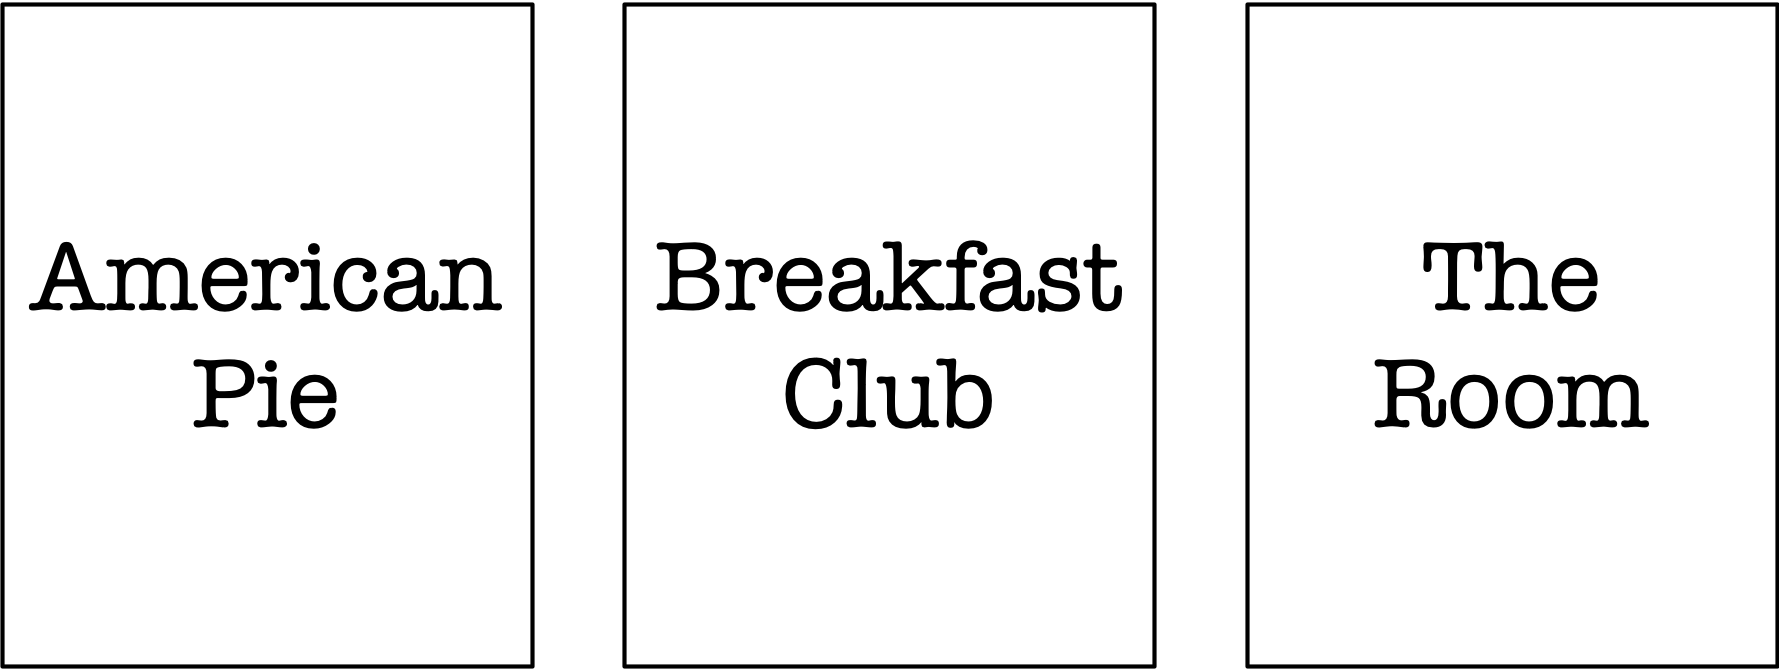
\includegraphics[width=\linewidth]{images/set_movies.png}
  \caption{Elements of set A.}
  \label{fig:marginfig}
\end{marginfigure}

A thing can be anything: name, object, idea. It's a very abstract notion. For example, I can define a set of movies I have seen: American Pie, Breakfast Club, The Room. Yes, I have only seen those three movies in my entire life. I am busy writing texts about set theory.

Actually, I've watched The Room five times. Does this affect the set? No, because it doesn't change the notion of "what movies I have watched". This obvious idea is an integral property of sets: they contain only unique objects.

\marginnote{Nothing stops us from defining a set of movie viewings, though. In that case, each element would be a particular instance of a "movie watching event", and, in my sad case, would contain 7 elements.}


If an object \(o\) is in set \(A\), we say \(o\) is a member of \(A\). To express this fact easily, mathematicians use the following notation: \(o \in A\).

So, if \(A = \textrm{Movies I've watched}\) and \(o = \textrm{The Room}\), then \(o \in A\). But if \(b = \textrm{Avengers}\),  then \(b \notin A\). Now you can generate infinitely many "nerdy" T-shirts with prints like \(\textrm{joy} \in \textrm{mylife}\) or \(\textrm{party} \in \textrm{dahouse}\).

If we were to look inside set \(A\), it might look like this:

\begin{equation}
\{s, m, o\}
\end{equation}

Sets don't have the notion of order, so it doesn't matter how you mention its members as long as you mention them all. So, all these:

\begin{itemize}
\item \(\{s, m, o\}\)
\item \(\{s, o, m\}\)
\item \(\{m, s, o\}\)
\item etc.
\end{itemize}

describe the same set \(A\).

We are lucky: set \(A\) is finite and quite small. But sets can be infinite, and it would be impossible to write down all of its members. There are ways to describe such sets nevertheless. For example, the set of all natural numbers from \(1\) to \(n\) can be described like so:

\begin{equation}
\{1, 2, 3, 4, ... n\}
\end{equation}

Here we rely on reader's common sense and assume he or she can rightfully deduce what is meant by the ellipsis (\texttt{...}). Notations like this are very common in math, and while it isn't awfully strict, the idea is to be as unambiguous as possible. For example, when describing a set of odd natural numbers from \(1\) to \(n\), this would be bad:

\begin{equation}
\{1, 3, ... n\}
\end{equation}

simply because the sample isn't long enough to make a single assumption.

Another example of a set that exists in math is the set of Boolean values:

\begin{equation}
\mathscr{B} = \{T, F\}
\end{equation}

\(T\) and \(F\) stand for \emph{True} and \emph{False}. Certain tests (or, in other words, questions) that can be answered with "yes" and "no", produce values of said set. So, we can say that

\begin{equation}
(x > y) \in \mathscr{B}, \textrm{where }  x \in \mathbb{N} \textrm{ and } y \in \mathbb{N}
\end{equation}

In other words, the answer to the question "is \(x\) greater than \(y\)" is a member of set \(\mathscr{B}\), as long as \(x\) and \(y\) are members of \(\mathbb{N}\) (i.e. natural numbers).

Math in infinitely composable. Most programming languages can only dream of the level of composability and flexibility mathematicians enjoy. While not immediately useful, we could compose the following statements about sets:

\begin{equation}
((x + y) \in \mathbb{N}) \in \mathscr{B}, \textrm{where }  x, y \in \mathbb{N}
\end{equation}

Here we said "when \(x\) and \(y\) are members of \(\mathbb{N}\), then the answer to the question 'is \(x + y\) a member of \(\mathbb{N}\)' is a member of \(\mathscr{B}\)."

Many groups in mathematics are sets: numbers of different types (natural, irrational, complex, etc.), notions of different types (e.g. Boolean), solutions to particular problems (e.g. graphs that satisfy a certain property). But describing groups of elements is just the tip of the iceberg. Set theory, with its axioms and definitions, can play a role of a foundational area of math, from which many other areas can be derived.

In this course and the book we're not going to talk about how set theory (and category theory) can "generate" a large portion of the whole math. But these topics are among the most fascinating frontiers of modern mathematics.

\section{Empty set}
\label{sec:org216fd5a}

Mathematicians love zero. Ever since its inception around 1770 BC, zero is an important part of mathematical models. The notion of "nothingness", which zero reflects in the context of counting, is present in all areas. In the context of sets, nothingness is an \emph{empty set}.

\begin{equation}
\varnothing = \{\}
\end{equation}

Why would we need empty sets? Well, sometimes we want to describe a notion of having no objects under a certain description. For example, since I only watched 3 movies in my life, and all of them were American, I can describe:

\begin{equation}
\varnothing = \textrm{the set of all non-American movies I've watched}.
\end{equation}

A more mathematical example would be something like this:

\begin{equation}
\varnothing = \{x | x \in \mathbb{N} \textrm{ and } x < 0\}
\end{equation}

which says that the set of natural numbers smaller than zero is an empty set. It's a formal way to say that there are no natural numbers less than zero.

Note the use of vertical line \textbf{\texttt{|}}, it is a shorter way to say "where".

\section{Subset, superset}
\label{sec:org1e2a9b1}

When all members of set \(A\) are present in another set \(B\), then \(A\) is a \textbf{subset} of \(B\). Let's say set \(B\) is the set of all movies ever produced. Then \(A\) (movies I've watched) is clearly a subset of \(B\). This notion is expressed like so:

\begin{equation}
A \subseteq B
\end{equation}

To look at things from the other end, \(B\) is a \textbf{superset} of \(A\):

\begin{equation}
B \supseteq A
\end{equation}

\begin{marginfigure}
  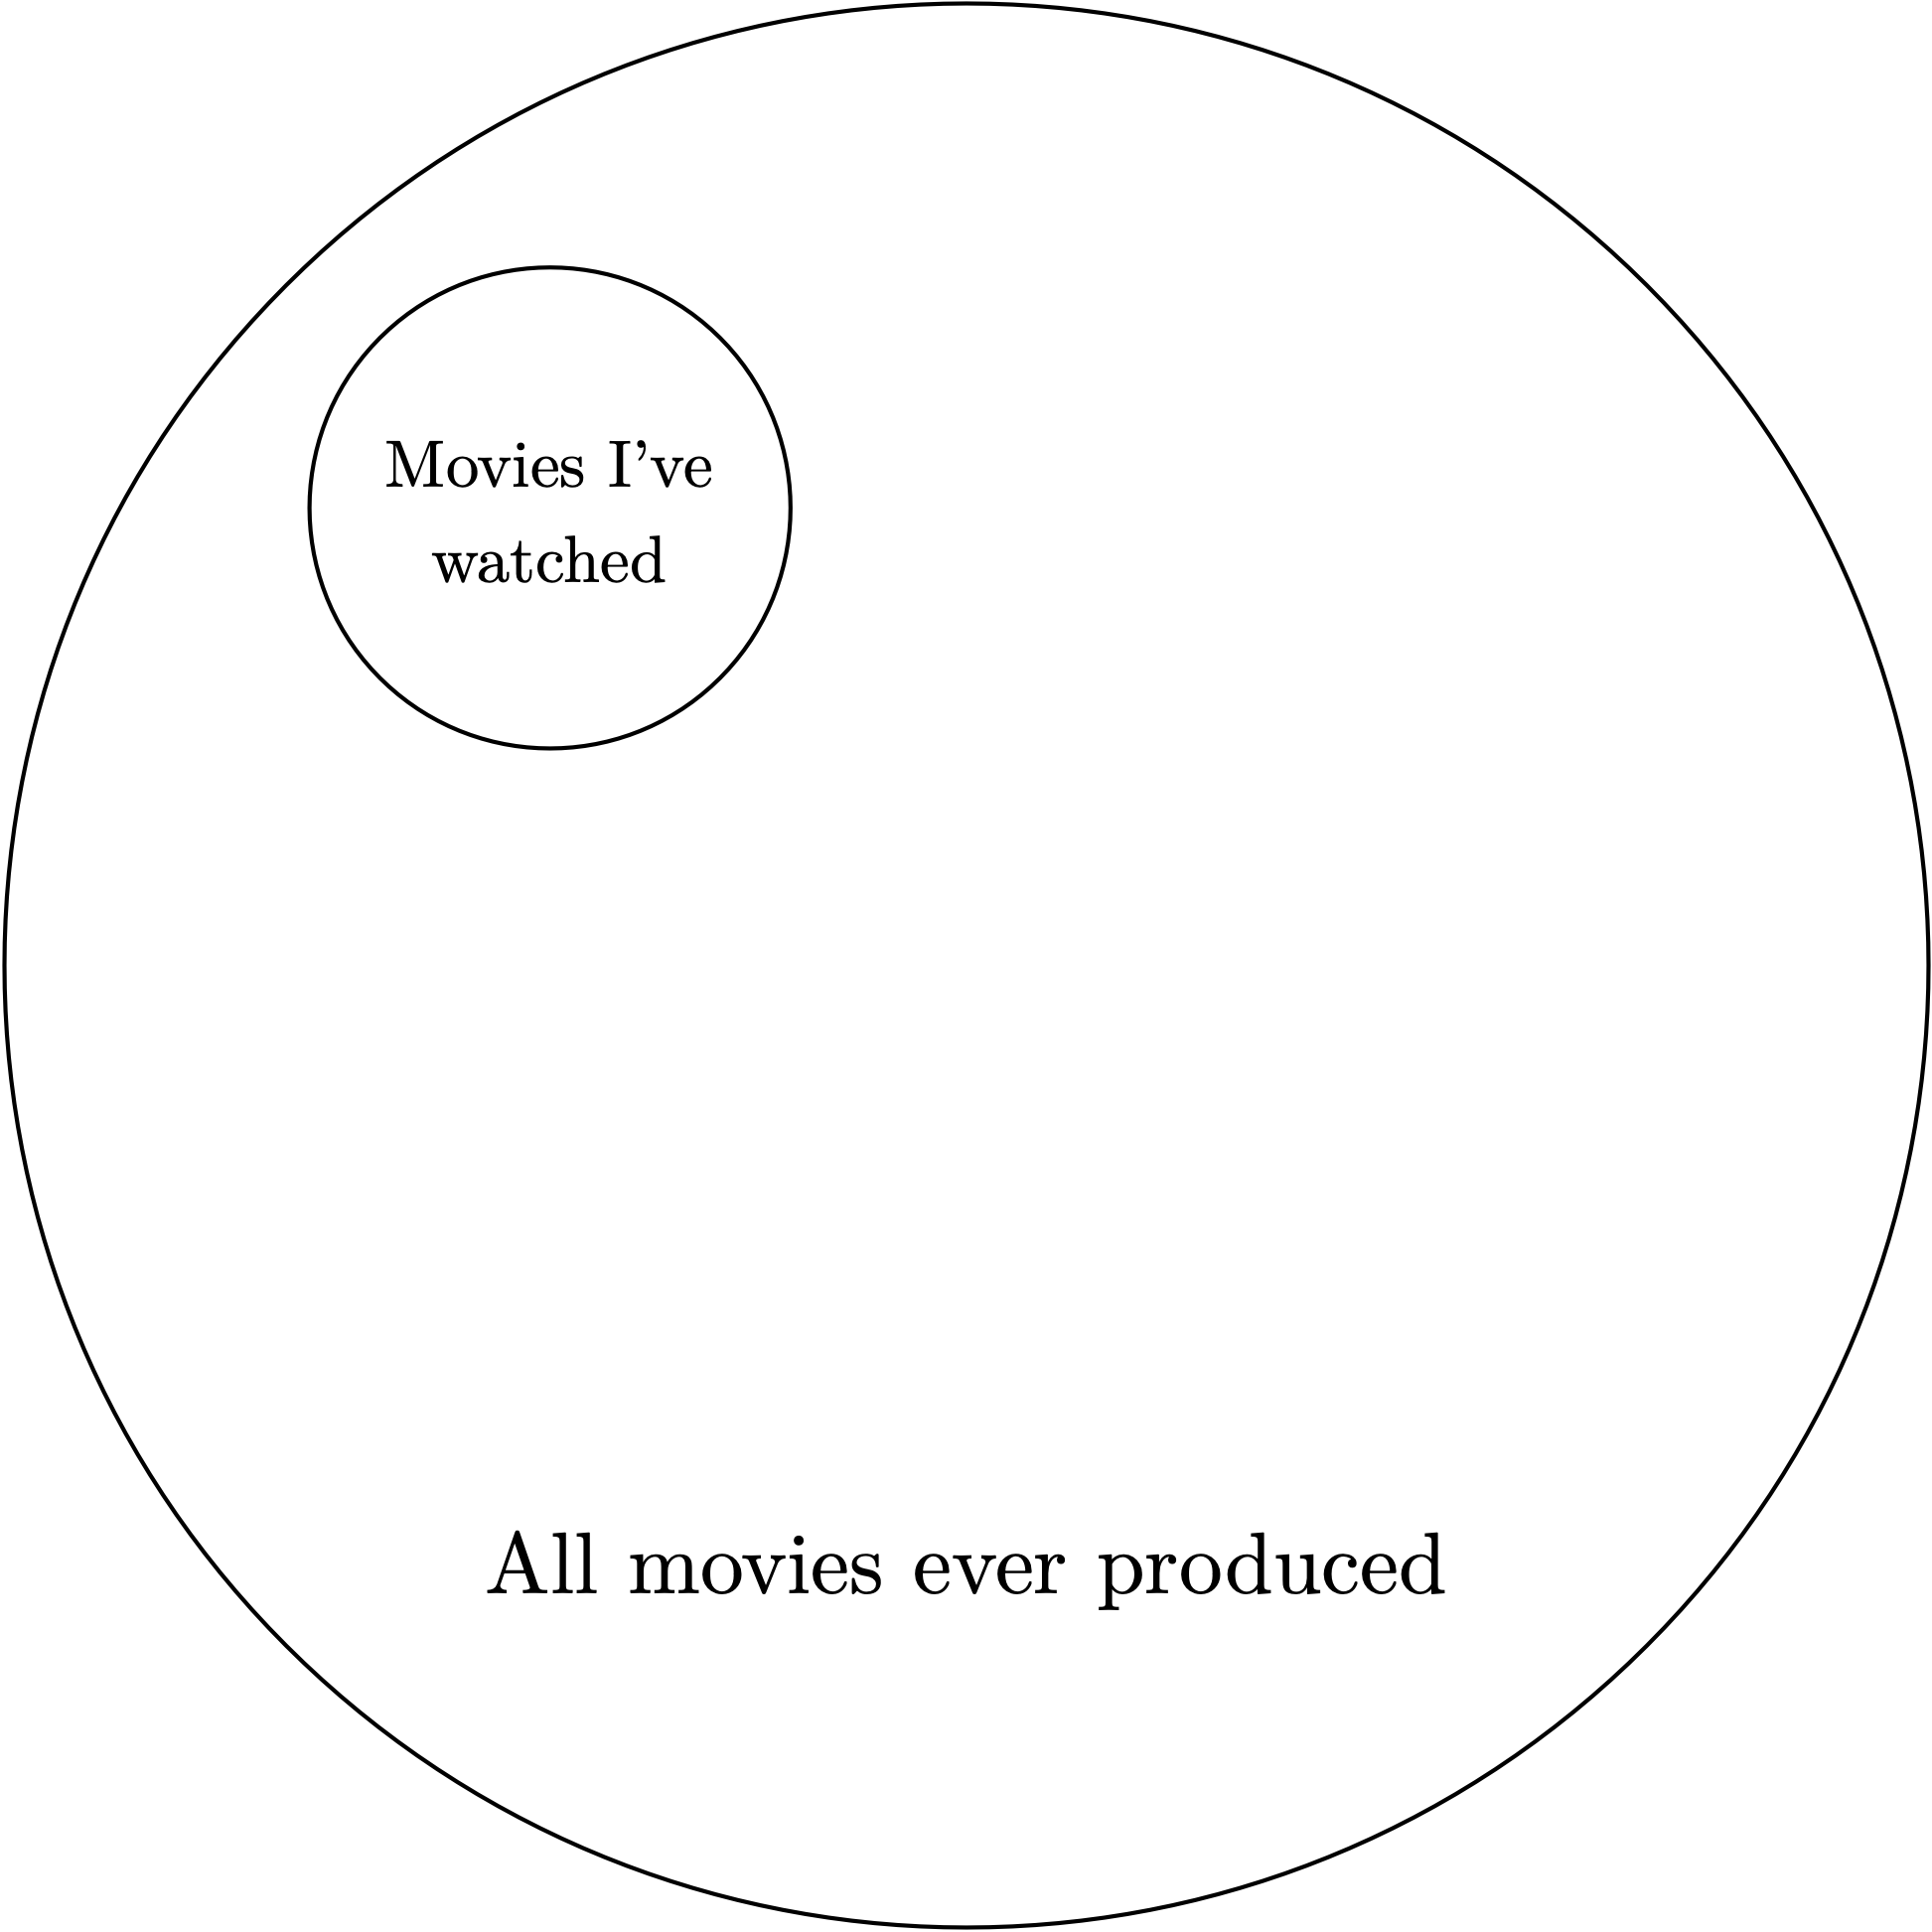
\includegraphics[width=\linewidth]{images/subset.png}
  \caption{A set and its subset.}
  \label{fig:marginfig}
\end{marginfigure}


You know what else is a subset of \(B\)? An empty set!

\begin{equation}
\varnothing \subseteq B
\end{equation}

This either sounds absolutely natural to you or extremely weird. It makes perfect sense to a mathematician, because it's easy to argue: \emph{all} members of \(\varnothing\) are present in \(B\), all zero of them.

It gets weirder. As per our definition, if all members of a set are also present in another set, then the one is a subset of the other. This means any set is a subset of itself.

\begin{equation}
\displaylines{
A \subseteq A \\
B \subseteq B \\
Z \subseteq Z
}
\end{equation}

By extension, if two sets are the same, then either of them is a subset of the other.

\begin{equation}
\textrm{if } A \subseteq B \textrm{ and } B \subseteq A \textrm{ then } A = B
\end{equation}

When we look at a statement \(A \subseteq B\), we often need to know whether \(A = B\) or not. To distinguish between the two cases, mathematicians use a special notion of a \textbf{proper subset}.

If \(A \in B\), but \(A \neq B\), then \(A\) is a proper subset of \(B\).

\begin{equation}
A \subset B
\end{equation}

Since I haven't watched all the movies ever produced, I can say that \(A\) is a proper subset of \(B\). So, a set is a subset of itself, but is never a proper subset of itself.

\section{Cardinality}
\label{sec:orgc592b33}

Before we start to talk about sizes and products, let's first introduce a new notion:  \textbf{\textbf{sequence}}. A sequence is simply a series of elements. Unlike sets, sequences have order and may contain duplicate values. In this sense sequences are more down to earth, practical collections.

Sequences are written with round brackets. For example, a sequence of prime numbers in ascending order is:

\begin{equation}
(2, 3, 5, 7, 11, ...)
\end{equation}

Note that it is an infinite sequence. An example of a finite sequence is a sequence of natural even numbers smaller than 10:

\begin{equation}
(1, 2, 3, 4, 5, 6, 7, 8, 9)
\end{equation}

\noindent\rule{\textwidth}{0.5pt}

If \(A\) is a finite set (that is, \(A\) is not infinite, and we can count how many elements there are in it), we use \(|A|\) to denote the number of elements of \(A\). This is the \textbf{\textbf{cardinality}}. For example:

\begin{equation}
\displaylines{
|\{4, 8, 15, 16, 23, 42\}| = 6, \\
|\varnothing| = 0, \\
|\{\{a, e\}\}| = 1.
}
\end{equation}

Note the last example: it defines a set which contains one set, thus its cardinality is 1. The number of elements of the internal set is irrelevant. Programmers find this obvious, as it reminds them of nested data structures like arrays of arrays.

Knowing about sets, subsets and cardinalities, let's look at a statement and prove it.

\textbf{Statement 1}: \emph{If \(A\) is a finite set of \(m\) elements, then there are \(2^{m}\) subsets of \(A\).}

\textbf{Proof}: Suppose \(A = \{a_{1}, a_{2}, ..., a_{m}\}\) and \(\mathscr{P}A\) is the set of all subsets of \(A\). Then we can divide \(\mathscr{P}A\) into \(2=2^{1}\) collections: subsets of \(A\) which contain \(a_{1}\) and those which don't. Considering the next element \(a_{2}\), we get 4=2\(^{\text{2}}\) collections:

\begin{enumerate}
\item One which contains both \(a_{1}\) and \(a_{2}\),
\item one which contains \(a_{1}\), but not \(a_{2}\),
\item one which contains \(a_{2}\), but not \(a_{1}\),
\item one which contains neither \(a_{1}\) nor \(a_{2}\).
\end{enumerate}

Continuing this way, we see that there are \(2^{m}\) subsets of \(A\), each subset is determined by the fact of whether or not each \(a_{j}\) is included, as \(j\) goes from \(1\) to \(m\).

This sort of counting by inclusion / exclusion is a popular technique in math and especially in computer science. One can visualize such proof for a particular case by drawing a "binary decision tree".

Consider set \(A = \{a_{1}, a_{2}, a_{3}\}\). The proof states that there are \(2^{3} = 8\) subsets of \(A\). Do describe each imaginable set we need to determine whether each element is in it or not. Starting from \(a_{1}\), we need to answer "yes" or "no", and proceed to ask the same question for \(a_{2}\) and then for \(a_{3}\).


\begin{figure*}[htbp]
\centering
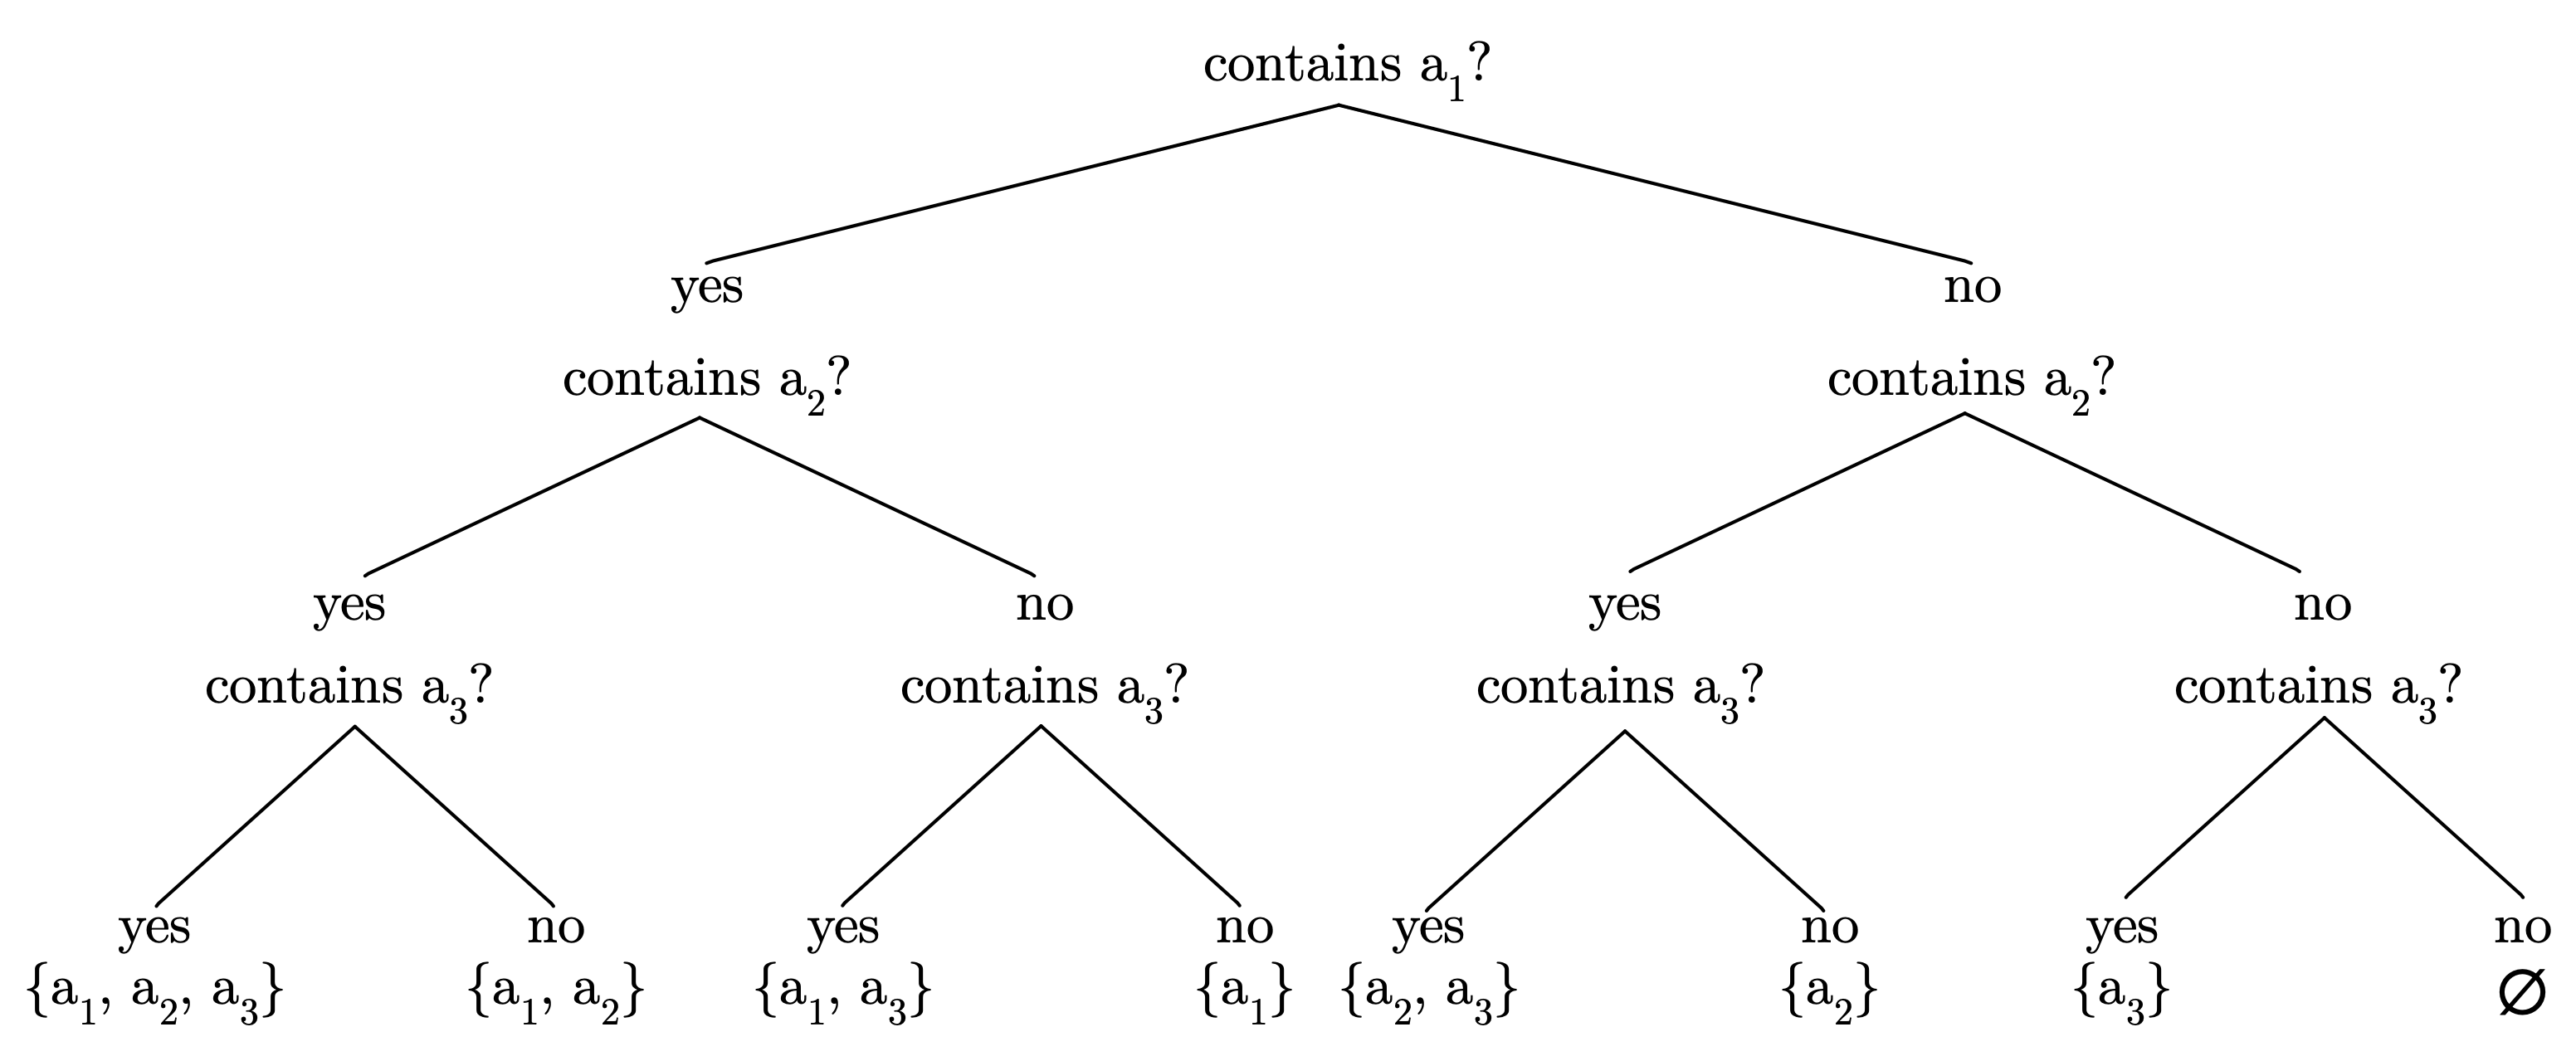
\includegraphics[width=.9\linewidth]{./images/powerset_binary_decision_tree.png}
\caption{\label{fig:orge2eb83a}
Binary decision tree for 8 subsets of \{a_{1}, a_{2}, a_{3}\}}
\end{figure*}

\section{Cartesian product}
\label{sec:org37f32b1}

Given two sets \(A\) and \(B\), we are often interested in all ordered pairs of their elements. For example, if \(A = \{a, b\}\) and \(B = \{1, 2\}\), the ordered pairs are as follows:

\begin{equation}
\displaylines{
(a, 1)\\
(a, 2)\\
(b, 1)\\
(b, 2)\\
}
\end{equation}

The set of all such pairs is called the \textbf{Cartesian product} of \(A\) and \(B\). The name comes from the French mathematician René Descartes.

\begin{marginfigure}
  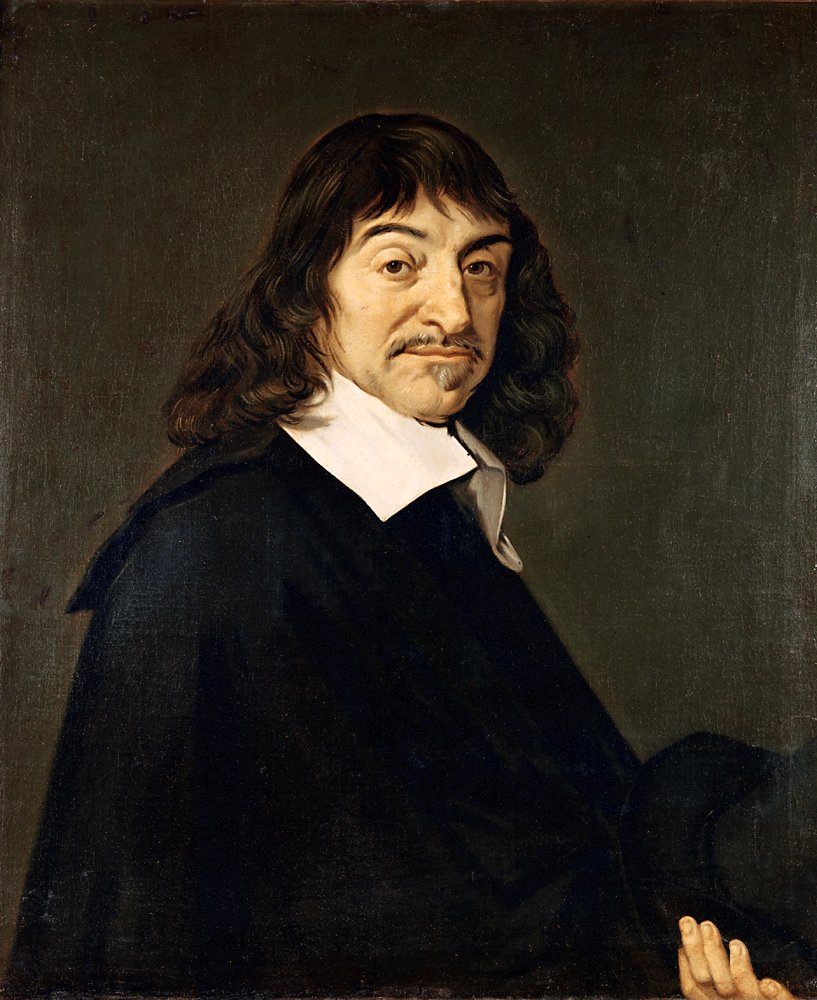
\includegraphics[width=\linewidth]{images/Frans_Hals_-_Portret_van_Rene_Descartes.jpg}
  \caption{Frans Hals, Portret van René Descartes}
  \label{fig:marginfig}
\end{marginfigure}

Formally, Cartesian product can be described like this:

\begin{equation}
A \times B = \{(a,b) | a \in A, b \in B\}
\end{equation}

Descartes saw that the number plane \(x, y\) could be represented as a product of two sets of real numbers.

\begin{equation}
\mathbb{R} \times \mathbb{R} = \{(x, y) | x \in \mathbb{R}, y \in \mathbb{R}\}
\end{equation}

\begin{figure}[htbp]
\centering
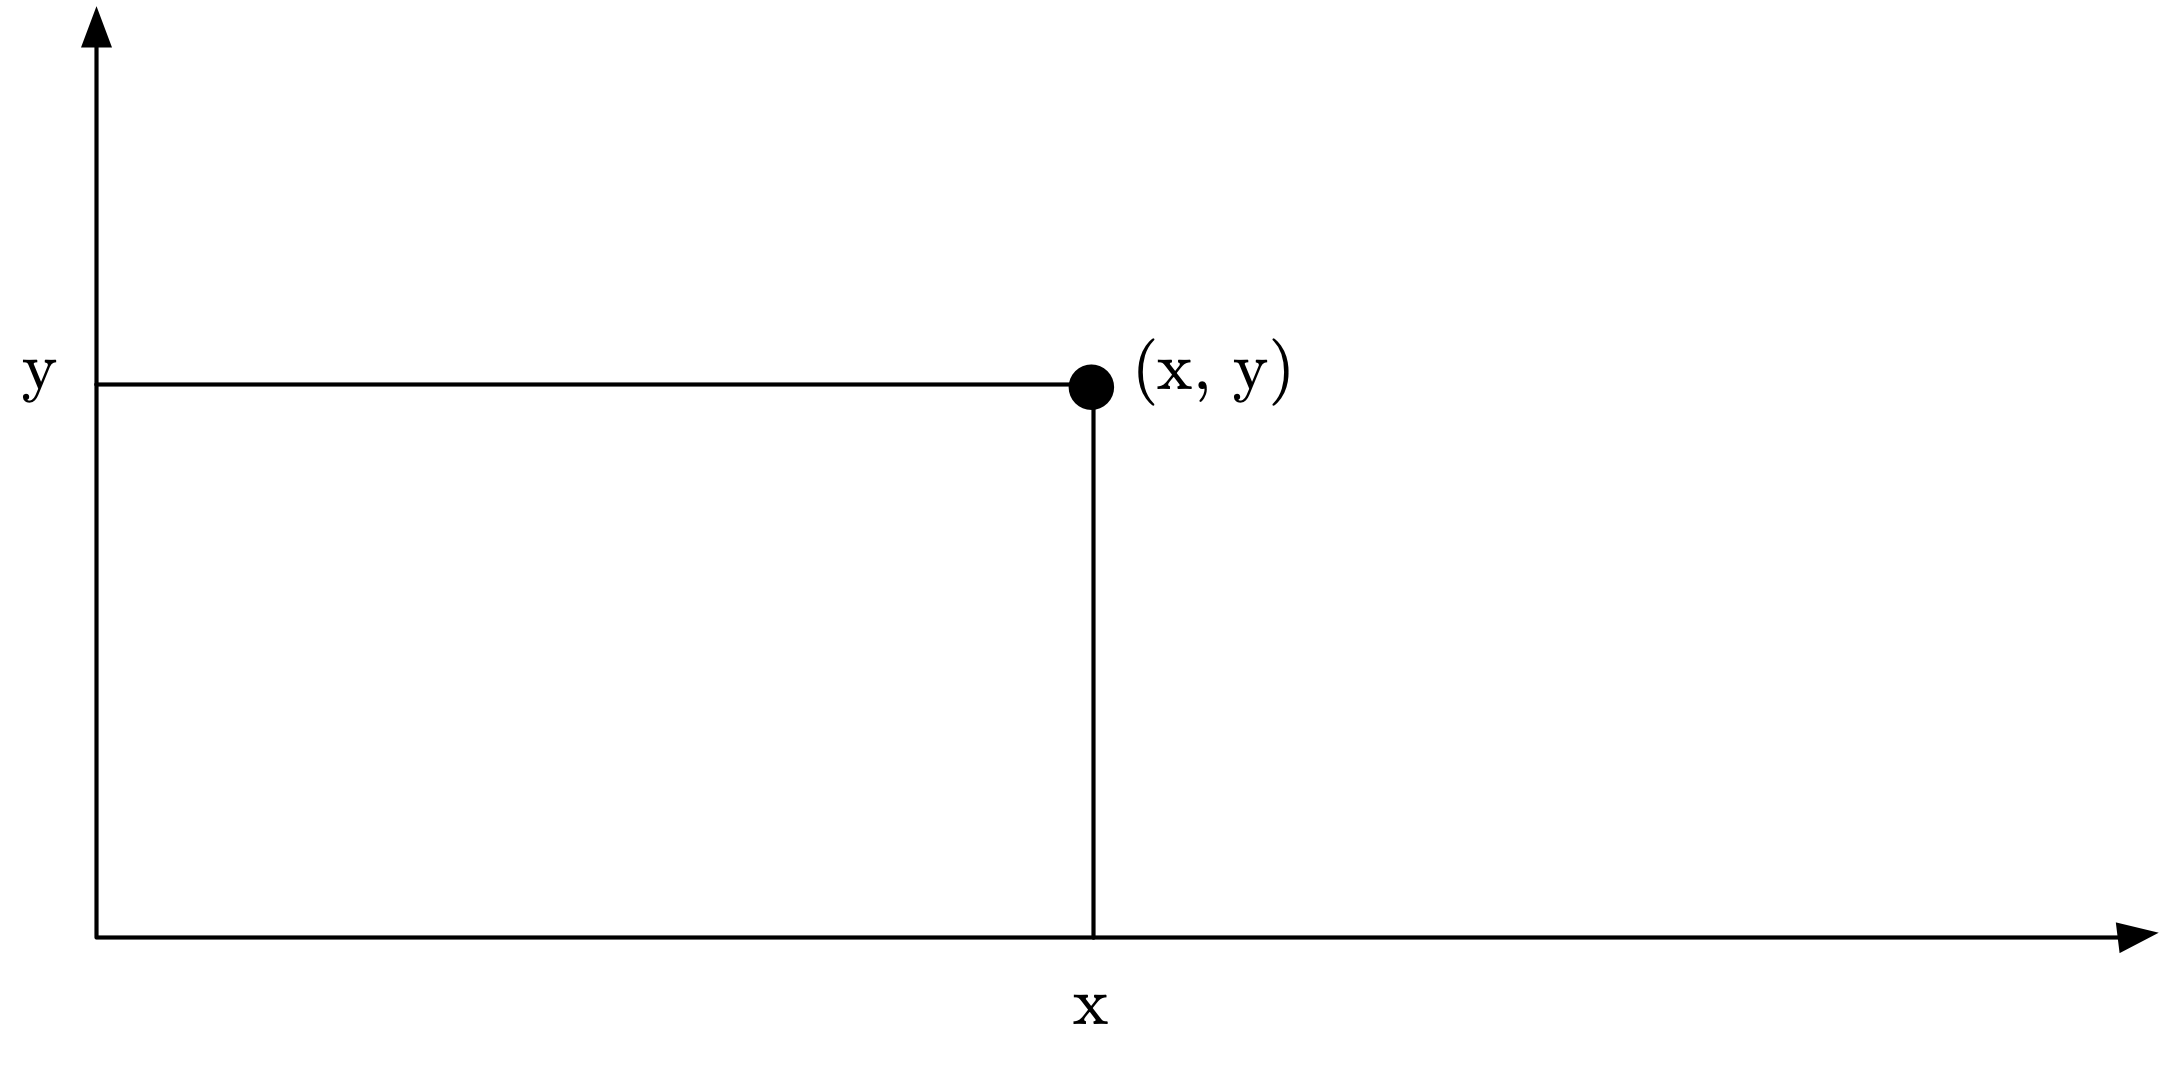
\includegraphics[width=.9\linewidth]{./images/xy_plane.png}
\caption{\label{fig:orge2eb83a}
Each point on x, y plane is in the Cartesian product of 2 sets of real numbers.}
\end{figure}

\section{Union}
\label{sec:org675db10}

Sets on their own are a bit boring, frozen things. Interesting results can be observed when we consider interactions between sets. At the same time, these interactions can be viewed as frozen things themselves, not actions or processes.

This happens often in math: the same idea can be viewed as either an action or a thing. Even functions, seemingly action-able, moving notions, can (and will) be defined as mere static constructs. It's interesting to ponder about these things, draw analogies to physics and time.

Regardless, let's quickly overview three main sorts of interactions. Chances are they are already very familiar to you, especially if you've done any SQL.

\textbf{\textbf{Union}} of a collection of sets is the set of all elements of the collection.

Given two sets \(A\) and \(B\), union is defined as:

\begin{equation}
A \cup B = \{ x : x \in A \textrm{ or } x \in B \}
\end{equation}

This reads as:

\begin{quote}
Union of \(A\) and \(B\) is a set of elements \(x\), where \(x\) belongs to \(A\) or x belongs to \(B\).
\end{quote}

For example, if \(A = \{1, 2, 3\}\), and \(B = \{3, 4, 5\}\), then:

\begin{equation}
A \cup B = \{1, 2, 3, 4, 5\}
\end{equation}

Note that even though each set contains 3 elements, the resulting union contains 5 elements only. Since union is a set, all rules and properties regarding sets still apply, so it cannot contain element \(3\) twice.

It is sometimes necessary to keep duplicates somehow, without violating the rules of sets. One way is "tag" each element in both sets by generating a Cartesian product of each set.

\begin{equation}
\displaylines{
A \times \{t_{A} \} = \{(1, t_{A}), (2, t_{A}), (3, t_{A}) \} \\
B \times \{t_{B} \} = \{(3, t_{B}), (4, t_{B}), (5, t_{B}) \}
}
\end{equation}

So now instead of each number we deal with a sequence of two elements: the original number and a tag which refers to the original set. We use the term \emph{n-tuple} for a sequence of length \(n\). Thus, here we deal with sets of \emph{2-tuples}.

Since all tuples are unique, the resulting union set contains 6 distinct elements:

\begin{equation}
\displaylines{
A \times \{t_{A} \} \cup B \times \{t_{B} \} = \\
\{(1, t_{A}), (2, t_{A}), (3, t_{A}), (3, t_{B}), (4, t_{B}), (5, t_{B}) \}
}
\end{equation}

Every time we learn about a new approach or an idea, your inner mathematician should aspire to generalize. We've already generalized the notion of union by providing a formal mathematical definition. Let us now define this so-called \textbf{\textbf{disjoint union}} \(\sum A_{i}\) to be:

\begin{equation}
\bigcup_{1 \leq i \leq n} A_{i} \times \{i\} = \{(x, i) | x \in A_{i} \textrm{ and } 1 \leq i \leq n\}
\end{equation}

It might seem like the notation is getting more and more complicated, but it's only a combination of existing notions and symbols, nothing new. The big U is a generalization of unions, here it is limited to all sets \(A_{i} \times \{i\}\) where \(i\) goes from 1 to some \(n\). You can think of \(i\) as a variable or a parameter. We see it is then used to define different sets (e.g. \(A_{1}\), \(A_{2}\), etc) and corresponding tagging sets \(\{1\}\), \(\{2\}\), etc. Then, on the right-hand side of the equation there's a set of many 2-tuples, each containing an element from \(A_{i}\) and a tagging number \(i\).

To easily differentiate between regular unions and disjoint unions, we use two different symbols: \(\cup\) for union, \(+\) for disjoint union. Thus:

\begin{equation}
\bigcup_{1 \leq i \leq n} A_{i} \times \{i\} = A_{1} + ... + A_{n}.
\end{equation}

\noindent\rule{\textwidth}{0.5pt}

Even if you haven't heard of set union, you've definitely seen Venn diagrams. They illustrate union, intersection and complement quite nicely.

\url{https://s3.amazonaws.com/thinkific/file\_uploads/146581/images/8cf/e18/857/British\_Isles\_Venn\_Diagram-en.svg.png}

Contrary to popular belief, Venn diagrams aren't suitable representations of \texttt{SQL JOIN}. You'll see why later.

When working with databases using SQL, union operation is a direct equivalent of union from set theory. The following example returns all usernames of both customers and managers:

\begin{verbatim}
SELECT username FROM users
UNION
SELECT username FROM managers;
\end{verbatim}

This regular \texttt{UNION} operation behaves like set union in regards to duplicates. Thus, if both tables contain identical usernames, only one instance would end up in the union. An alternative SQL operator \texttt{UNION ALL} allows duplicates. The resulting collection of records is not necessarily a set, since it main contain identical records.

It is tempting to see SQL as set theory applied to databases, but it would be wrong to think this way. SQL can be considered a domain specific language for a particular application of relational algebra, which \emph{incorporates} certain areas of set theory. In general, one can say that set theory and SQL \emph{intersect}.

\section{Intersection}
\label{sec:org7e00705}

\textbf{\textbf{Intersection}} of two sets \(A\) and \(B\) is the set containing all elements of \(A\) that also belong to \(B\) (or vice versa). In other words, it's a set of common elements.

\begin{equation}
A \cap B = \{ x : x \in A \textrm{ and } x \in B \}
\end{equation}

This reads as:

\begin{quote}
Intersection of \(A\) and \(B\) is the set of elements \(x\), where \(x\) belongs to \(A\) and x belongs to \(B\).
\end{quote}

For example, if \(A = \{1, 2, 3\}\), and \(B = \{3, 4, 5\}\), then 3 is the only element present in both sets:

\begin{equation}
A \cap B = \{3\}
\end{equation}

\emph{Sidenote: I quickly remembered which symbol -- \(\cup\) and \(\cap\) -- means which operation by noticing that \(\cup\) looks like letter U, so it means union. I've had a similar moment when learning Boolean algebra and logic, where \(\wedge\) means AND and looks like \(A\) without the horizontal bar.}

SQL has \texttt{INTERSECT}:

\begin{verbatim}
SELECT username FROM customers
INTERSECT
SELECT username FROM managers;
\end{verbatim}

Naturally, duplicates aren't an issue for intersection, because by definition one pair of elements results in one element, and not two. If there are two elements in one set, and one same element in the other set, the result is still one common element in the intersection.

A Venn diagram for intersection is often used to show commonality. For example, coming back to sets of favorite movies, we can compare your favorite movies and mine and see if there are any movies we both love. If no such movies exist, then our sets are \textbf{\textbf{disjoint}}. Formally, two sets are disjoint if their intersection is an empty set:

\begin{equation}
A \cap B = \varnothing
\end{equation}

A mathematician in love may describe the perfectness of their partner by saying that the partner's qualities and bad qualities are disjoint sets. The partner would definitely accept this as a complement.

\section{Complement (difference)}
\label{sec:org2e32783}

\textbf{\textbf{Complement}} of set \(A\) is a set of elements not in \(A\). In other words, it's the opposite of \(A\).

\begin{equation}
A^{C} = \{x : x \notin A \}
\end{equation}

The notion of complement (or difference) requires an implicit assumption: what other elements are we talking about? Say, the complement of all positive numbers is negative numbers, and zero, and dogs, and Korean words, and\ldots{} all possible elements that aren't positive numbers? Thinking this way quickly reduces the conversation to either absurdity or to Russell's paradox. This is why the complement assumes some larger set in which \(A\) exists. This larger set should be obvious from the context, or should be specified explicitly somewhere. For instance, when talking about movies, the complement of the set of my favorite movies is obviously all other movies that aren't my favorite.

The term \textbf{universe} is used for a collection of entities one wishes to consider. For the example of movies, the universe is probably "all movies ever produced".

\noindent\rule{\textwidth}{0.5pt}

It's sometimes useful to consider the complement of a set with respect to some other well-defined set. This is often called \textbf{set difference} and is denoted as \(A - B\). Formally:

\begin{equation}
A - B = \{x | x \in A \textrm{ but } x \notin B\}
\end{equation}

SQL operator \texttt{EXCEPT} is similar to this idea.

\begin{verbatim}
SELECT username FROM users
EXCEPT
SELECT username FROM managers;
\end{verbatim}

This query would return all users who aren't managers. In set theory, we'd write it this way:

\begin{equation}
\textrm{Users} - \textrm{Managers}
\end{equation}

Or, with implicit universe:

\begin{equation}
\textrm{Managers}^{C}
\end{equation}

with an assumption that we're talking about users in general.

\section{Relational algebra}
\label{sec:orgee6c250}

If you worked with SQL in different databases, you might've noticed slight differences or even large, annoying discrepancies. The reason is that SQL isn't a formal, strict language, but rather an approach based on a general formal language called Relational algebra. Developers of different databases design their own versions of SQL and implement and modify its features at their discretion.

Relational algebra was created by Edgar F. Codd in 1960s-1970s, who worked at IBM at the time. Codd proposed this formal language as a basis for database querying.

The good news is that knowing set theory and relational algebra reduces potential SQL-related problems to basically documentation lookup. If you know how unions work, what's the idea behind a Cartesian product and what are expressions of relational algebra, then it comes down to finding the correct SQL syntax to solve the problem at hand.

We will finish up the section on set theory with a short overview of different aspects of relational algebra and their relation to SQL.

\begin{enumerate}
\item Relation
\label{sec:org9ba77e4}

\textbf{\textbf{Relation}} is essentially a table, with columns (called "attributes") and rows. For example, a relation \texttt{User} may be used to describe users in a web service.

\begin{verbatim}
User(id, username, firstName, lastName, email)
\end{verbatim}

\begin{center}
\begin{tabular}{rllll}
id & username & firstName & lastName & email\\
\hline
1 & jenn & Jenn & Clarkson & jnc@hotmail.com\\
2 & pax & Paxi & Romanov & paxro@aol.com\\
91 & thankso & Barack & Liu & bl@wh.gov\\
\end{tabular}
\end{center}

For demonstrating purposes, let's define another table:

\begin{verbatim}
Manager(id, department, level)
\end{verbatim}

\begin{center}
\begin{tabular}{rlr}
id & department & level\\
\hline
1 & engineering & 3\\
2 & medicine & 2\\
91 & mathematics & 3\\
\end{tabular}
\end{center}

The name of a relation can play a role of the simplest query:

\begin{verbatim}
User
\end{verbatim}

which returns the whole table.

\item Projection
\label{sec:org0e8f5e9}

A \textbf{\textbf{projection}} is an operation of extracting records with specific columns (attributes). It is denoted by Greek letter \(\Pi\) (uppercase pi), with a list of columns as subscript, followed by relation's name.

For example, here we extract a sub-relation of User with ids and emails only:

\begin{equation}
\Pi_{\textrm{id, email}} \textrm{ User}
\end{equation}

\begin{center}
\begin{tabular}{rl}
id & email\\
\hline
1 & jnc@hotmail.com\\
2 & paxro@aol.com\\
91 & bl@wh.gov\\
\end{tabular}
\end{center}

\item Select
\label{sec:orgf18b051}

A \textbf{\textbf{selection}} is an operation of filtering records by values. It is denoted by Greek letter \(\sigma\) (sigma) with a condition, followed by relation's name.

For example, here we get managers with level higher than 2:

\begin{equation}
\sigma_{\textrm{level} > 2} \textrm{ Manager}
\end{equation}

\begin{center}
\begin{tabular}{rlr}
id & department & level\\
\hline
1 & engineering & 3\\
2 & medicine & 2\\
91 & mathematics & 3\\
\end{tabular}
\end{center}

\item Operating on expressions
\label{sec:orgb48c8b7}

Select and project operators work on any expression, not only on whole relations. This means we can combine them arbitrarily. For example, we can select (essentially, filter) first, and then extract certain columns.

\begin{equation}
\Pi_{\textrm{id, level}} (\sigma_{\textrm{level} > 2} \textrm{ Manager})
\end{equation}

The result is a newly constructed relation consisting of only two columns, which, in turn, can be used for other operations:

\begin{center}
\begin{tabular}{rr}
id & level\\
\hline
1 & 3\\
91 & 3\\
\end{tabular}
\end{center}

\item Cross product (cartesian product)
\label{sec:orga4b2558}

Recall the idea behind Cartesian product in set theory: given two sets \(A = \{a, b\}\) and \(B = \{1, 2\}\), the \textbf{Cartesian product} is a set of pairs of all combinations of elements:

\begin{equation}
\displaylines{
(a, 1)\\
(a, 2)\\
(b, 1)\\
(b, 2)\\
}
\end{equation}

Much of the power of relational algebra comes from applying this idea to relations. It is also often called \textbf{cross product}.

Here's the cross-product of \texttt{User} and \texttt{Manager}:

\begin{equation}
\textrm{User} \times \textrm{Manager}
\end{equation}

\begin{center}
\begin{tabular}{rllllrlr}
User.id & username & firstName & lastName & email & Manager.id & department & level\\
\hline
1 & jenn & Jenn & Clarkson & jnc@hotmail.com & 1 & engineering & 3\\
1 & jenn & Jenn & Clarkson & jnc@hotmail.com & 2 & medicine & 2\\
1 & jenn & Jenn & Clarkson & jnc@hotmail.com & 91 & mathematics & 3\\
2 & pax & Paxi & Romanov & paxro@aol.com & 1 & engineering & 3\\
2 & pax & Paxi & Romanov & paxro@aol.com & 2 & medicine & 2\\
2 & pax & Paxi & Romanov & paxro@aol.com & 91 & mathematics & 3\\
91 & thankso & Barack & Liu & bl@wh.gov & 1 & engineering & 3\\
91 & thankso & Barack & Liu & bl@wh.gov & 2 & medicine & 2\\
91 & thankso & Barack & Liu & bl@wh.gov & 91 & mathematics & 3\\
\end{tabular}
\end{center}

Since both relations contain a column named \texttt{id}, the resulting relation contains two distinct columns with tagged names \texttt{User.id} and \texttt{Manager.id}. This is similar to the way we "tagged" items in set union.

This might not seem too useful: we just combined all records, and many of the new rows don't make sense. Cross-product is rarely useful as is. Instead, the goal is often to generate raw data for the operations. For example, with this long table at hand, we can first eliminate the nonsense rows by applying select:

\begin{equation}
\sigma_{\textrm{User.id} = \textrm{Manager.id}} (\textrm{User} \times \textrm{Manager})
\end{equation}


\begin{center}
\begin{tabular}{rllllrlr}
User.id & username & firstName & lastName & email & Manager.id & department & level\\
\hline
1 & jenn & Jenn & Clarkson & jnc@hotmail.com & 1 & engineering & 3\\
2 & pax & Paxi & Romanov & paxro@aol.com & 2 & medicine & 2\\
91 & thankso & Barack & Liu & bl@wh.gov & 91 & mathematics & 3\\
\end{tabular}
\end{center}

Assuming user ids in the system are used to identify managers as well, we now have a sensible relation of managers with their complete user info intact.

Now we can filter managers by level and get rid of unneeded columns:


\begin{equation}
\Pi_{\textrm{User.id, email, department}}
\big(
\sigma_{\textrm{User.id} = \textrm{Manager.id}, \textrm{level} > 2} (\textrm{User} \times \textrm{Manager})
\big)
\end{equation}

\begin{center}
\begin{tabular}{rll}
User.id & email & department\\
\hline
1 & jnc@hotmail.com & engineering\\
91 & bl@wh.gov & mathematics\\
\end{tabular}
\end{center}

\item Natural join
\label{sec:orge575251}

The process of performing a cross-product and then filtering out rows that "make sense" by comparing the attributes of the same name is common enough so that relational algebra has a special operator called \textbf{natural join}. It is denoted by \(\bowtie\) (bow tie). The result is a relation with matching rows and no "tagged" attributes:

\begin{equation}
\textrm{User} \bowtie \textrm{Manager}
\end{equation}

\begin{center}
\begin{tabular}{rlllllr}
id & username & firstName & lastName & email & department & level\\
\hline
1 & jenn & Jenn & Clarkson & jnc@hotmail.com & engineering & 3\\
2 & pax & Paxi & Romanov & paxro@aol.com & medicine & 2\\
91 & thankso & Barack & Liu & bl@wh.gov & mathematics & 3\\
\end{tabular}
\end{center}

As you see, natural join is basically a syntactic sugar on top of existing features of relational algebra.

\item Union, intersection, difference
\label{sec:org0f63a39}

Relational algebra includes three operators straight from set theory: union, intersection and difference. They work just like you might expect, although there are some caveats. We will not focus on these topics at the moment.
\end{enumerate}

\section{Relations and Functions}
\label{sec:orgbe9e5dd}

In programming, we often deal with paired data:

\begin{itemize}
\item username — email
\item person — phone number
\item id — company
\end{itemize}

All cases can be considered as two sets, with a rule to connect their elements.

Given two sets \(A\) and \(B\), a \emph{map function} \(f\) from \(A\) to \(B\), denoted as

\begin{equation}
f: A \rightarrow B
\end{equation}

is an assignment  to each element \(a\) in \(A\) of a single element in \(B\).

We sometimes use a notation \(a \mapsto f(a)\) (note the different arrow) to indicate that \(a\) maps to some value via function \(f\). We call \(f(a)\) an \emph{image} of \(a\). Set \(A\) is called the \emph{domain} of \(f\), and \(B\) the \emph{codomain} of \(f\).

Notice how we talk about functions as static data, not as a process. In programming, we're used to functions being descriptions of processes, even though in most languages we can pass functions around as data. But consider this: how would you cache a function call? An obvious approach is to pre-compute some answers beforehand and store them in a table:

\begin{center}
\begin{tabular}{lr}
Argument & Return\\
\hline
"a" & 52321\\
"b" & 12321\\
"c & 81872\\
\ldots{} & \ldots{}\\
\end{tabular}
\end{center}

Theoretically, we could do this for all possible arguments, which would allow us to disregard all function's code and continue operating with a cache table exclusively. This means that any function (unless it deals with randomization) can be represented as static data. A mathematical notation of a function as a relation between two sets (essentially, a set of arguments and a set of return values) generalizes this idea.

A \textbf{binary relation} of two sets \(A\) and \(B\) is a subset of \(A \times B\). (Recall that \(A \times B\) is a set of all combinations of pairs of values of the two sets). Thus, a \emph{function} is a binary relation, having the property that for each element \(a \in A\) there is exactly one ordered pair in \(A \times B\) whose first component is \(a\).

There are three types of relations:

\textbf{1.} The function \(f: A \rightarrow B\) is \emph{one-to-one} (\textbf{injective}) if no two values of \(A\) result in the same value of \(B\). In other words, there's at most one incoming arrow for each element of \(B\).

Formally: for any two distinct elements \(a\) and \(a'\) in \(A\), we have \(f(a) \neq f(a')\).

\begin{figure}
  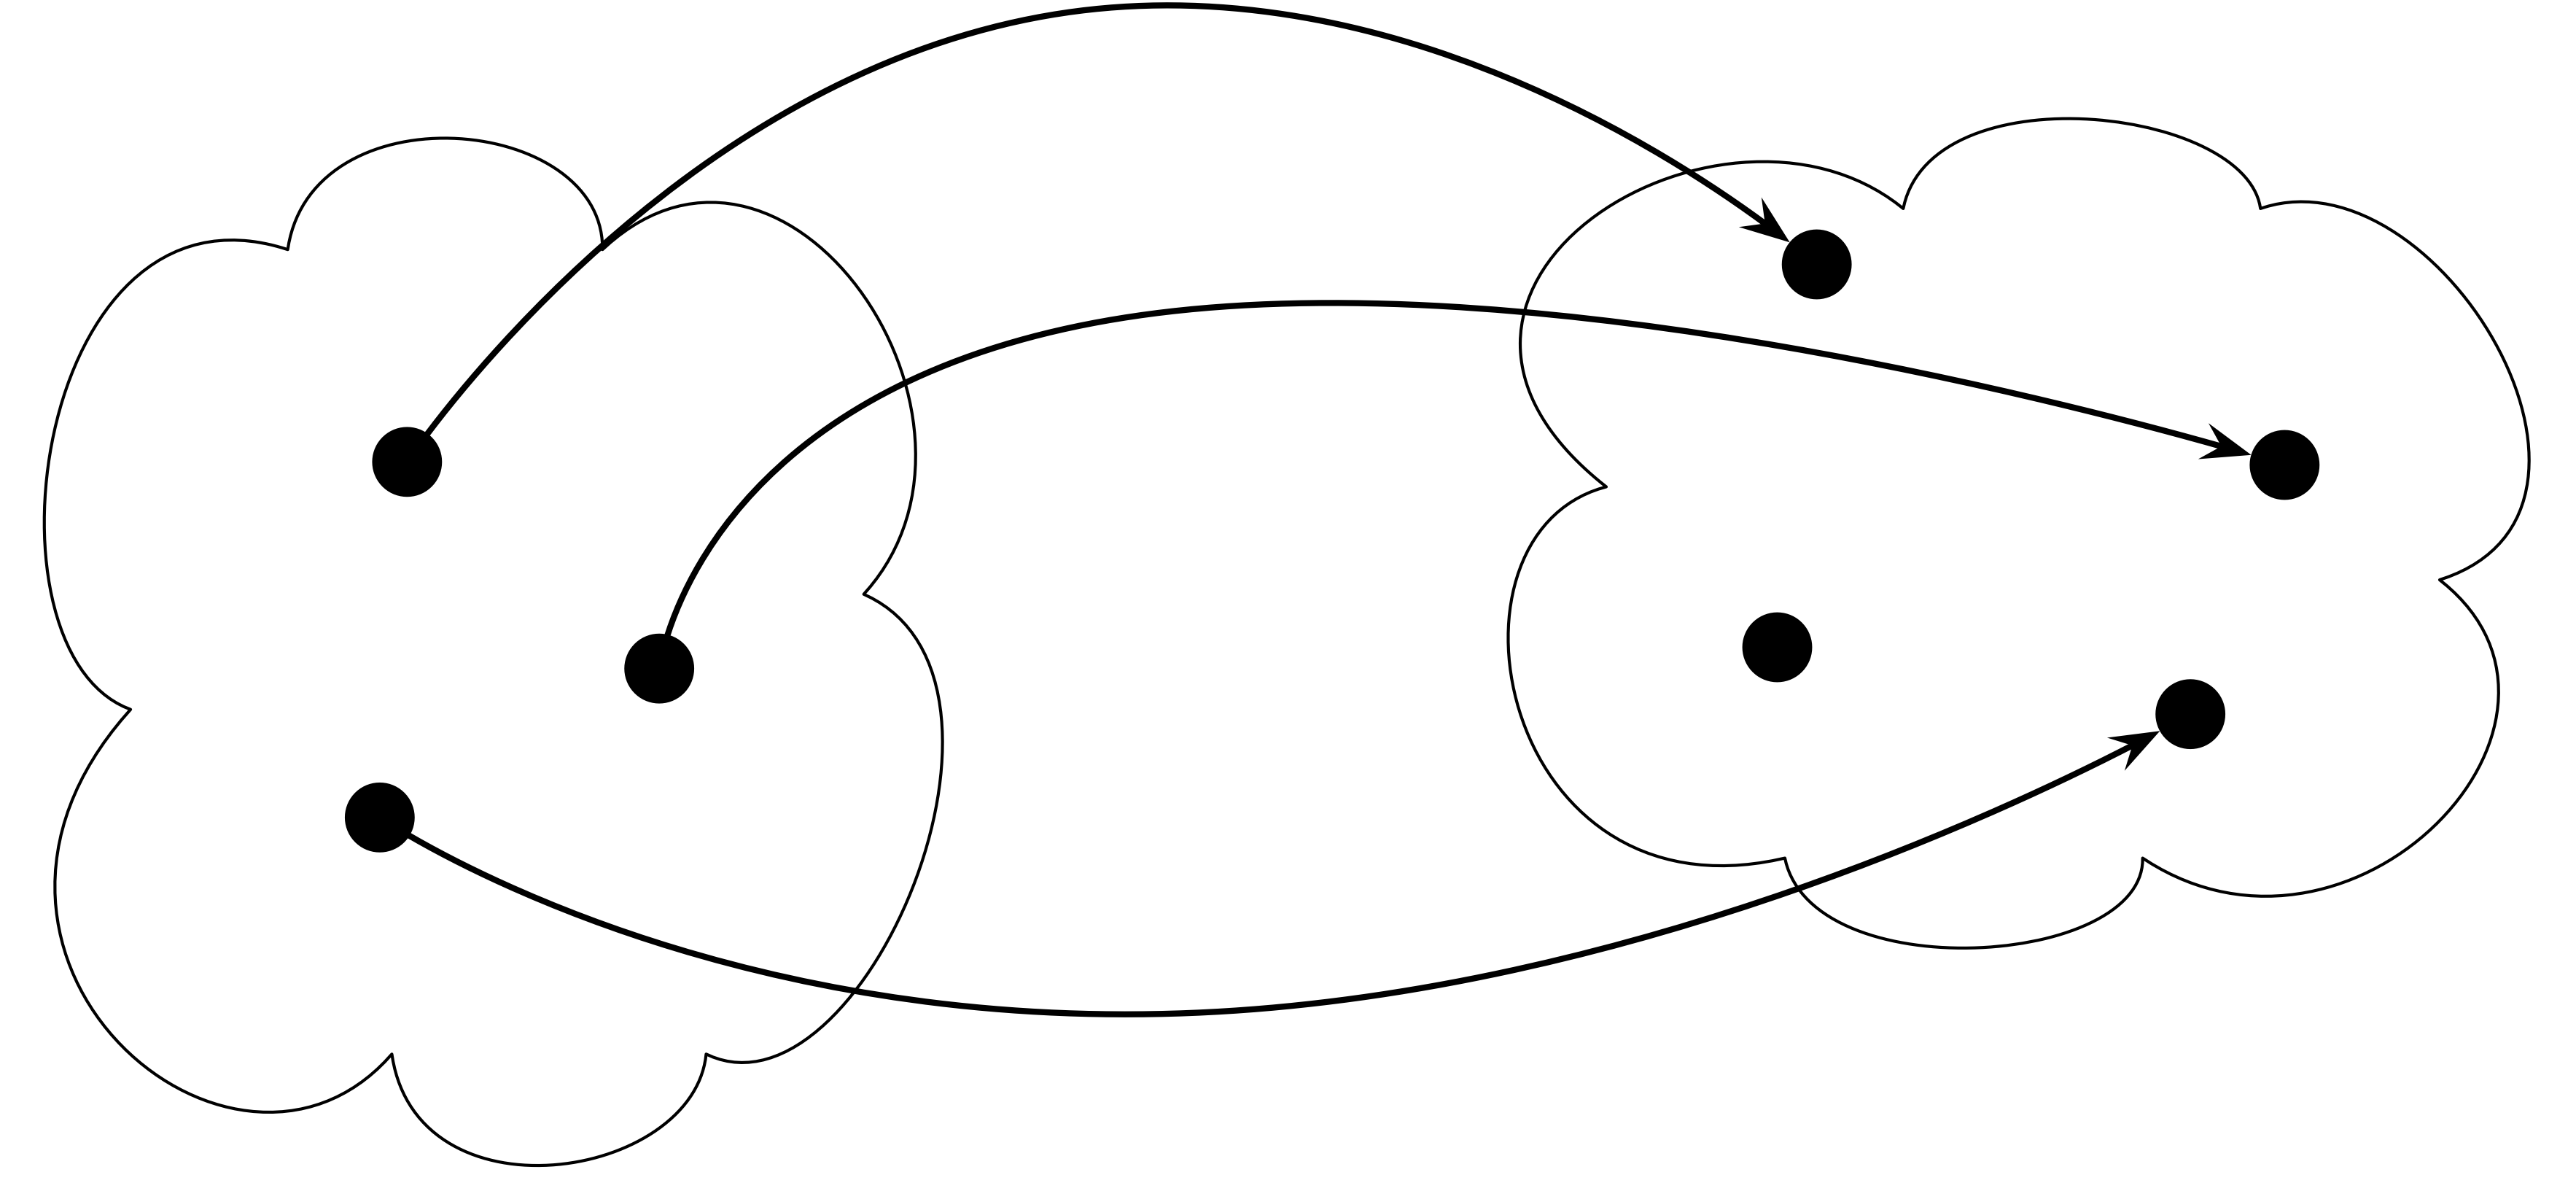
\includegraphics[width=.5\linewidth,right]{images/relations/injection.png}
  \caption{Injection.}
  \label{fig:injection}
\end{figure}

\textbf{2.} The function \(f: A \rightarrow B\) is \emph{onto} (\textbf{surjective}) if all elements of \(B\) are covered. In other words, no element of \(B\) is without at least one arrow.

Formally: for each element \(b \in B\), there exists an element \(a \in A\), such that \(f(a) = b\).

\begin{figure}
  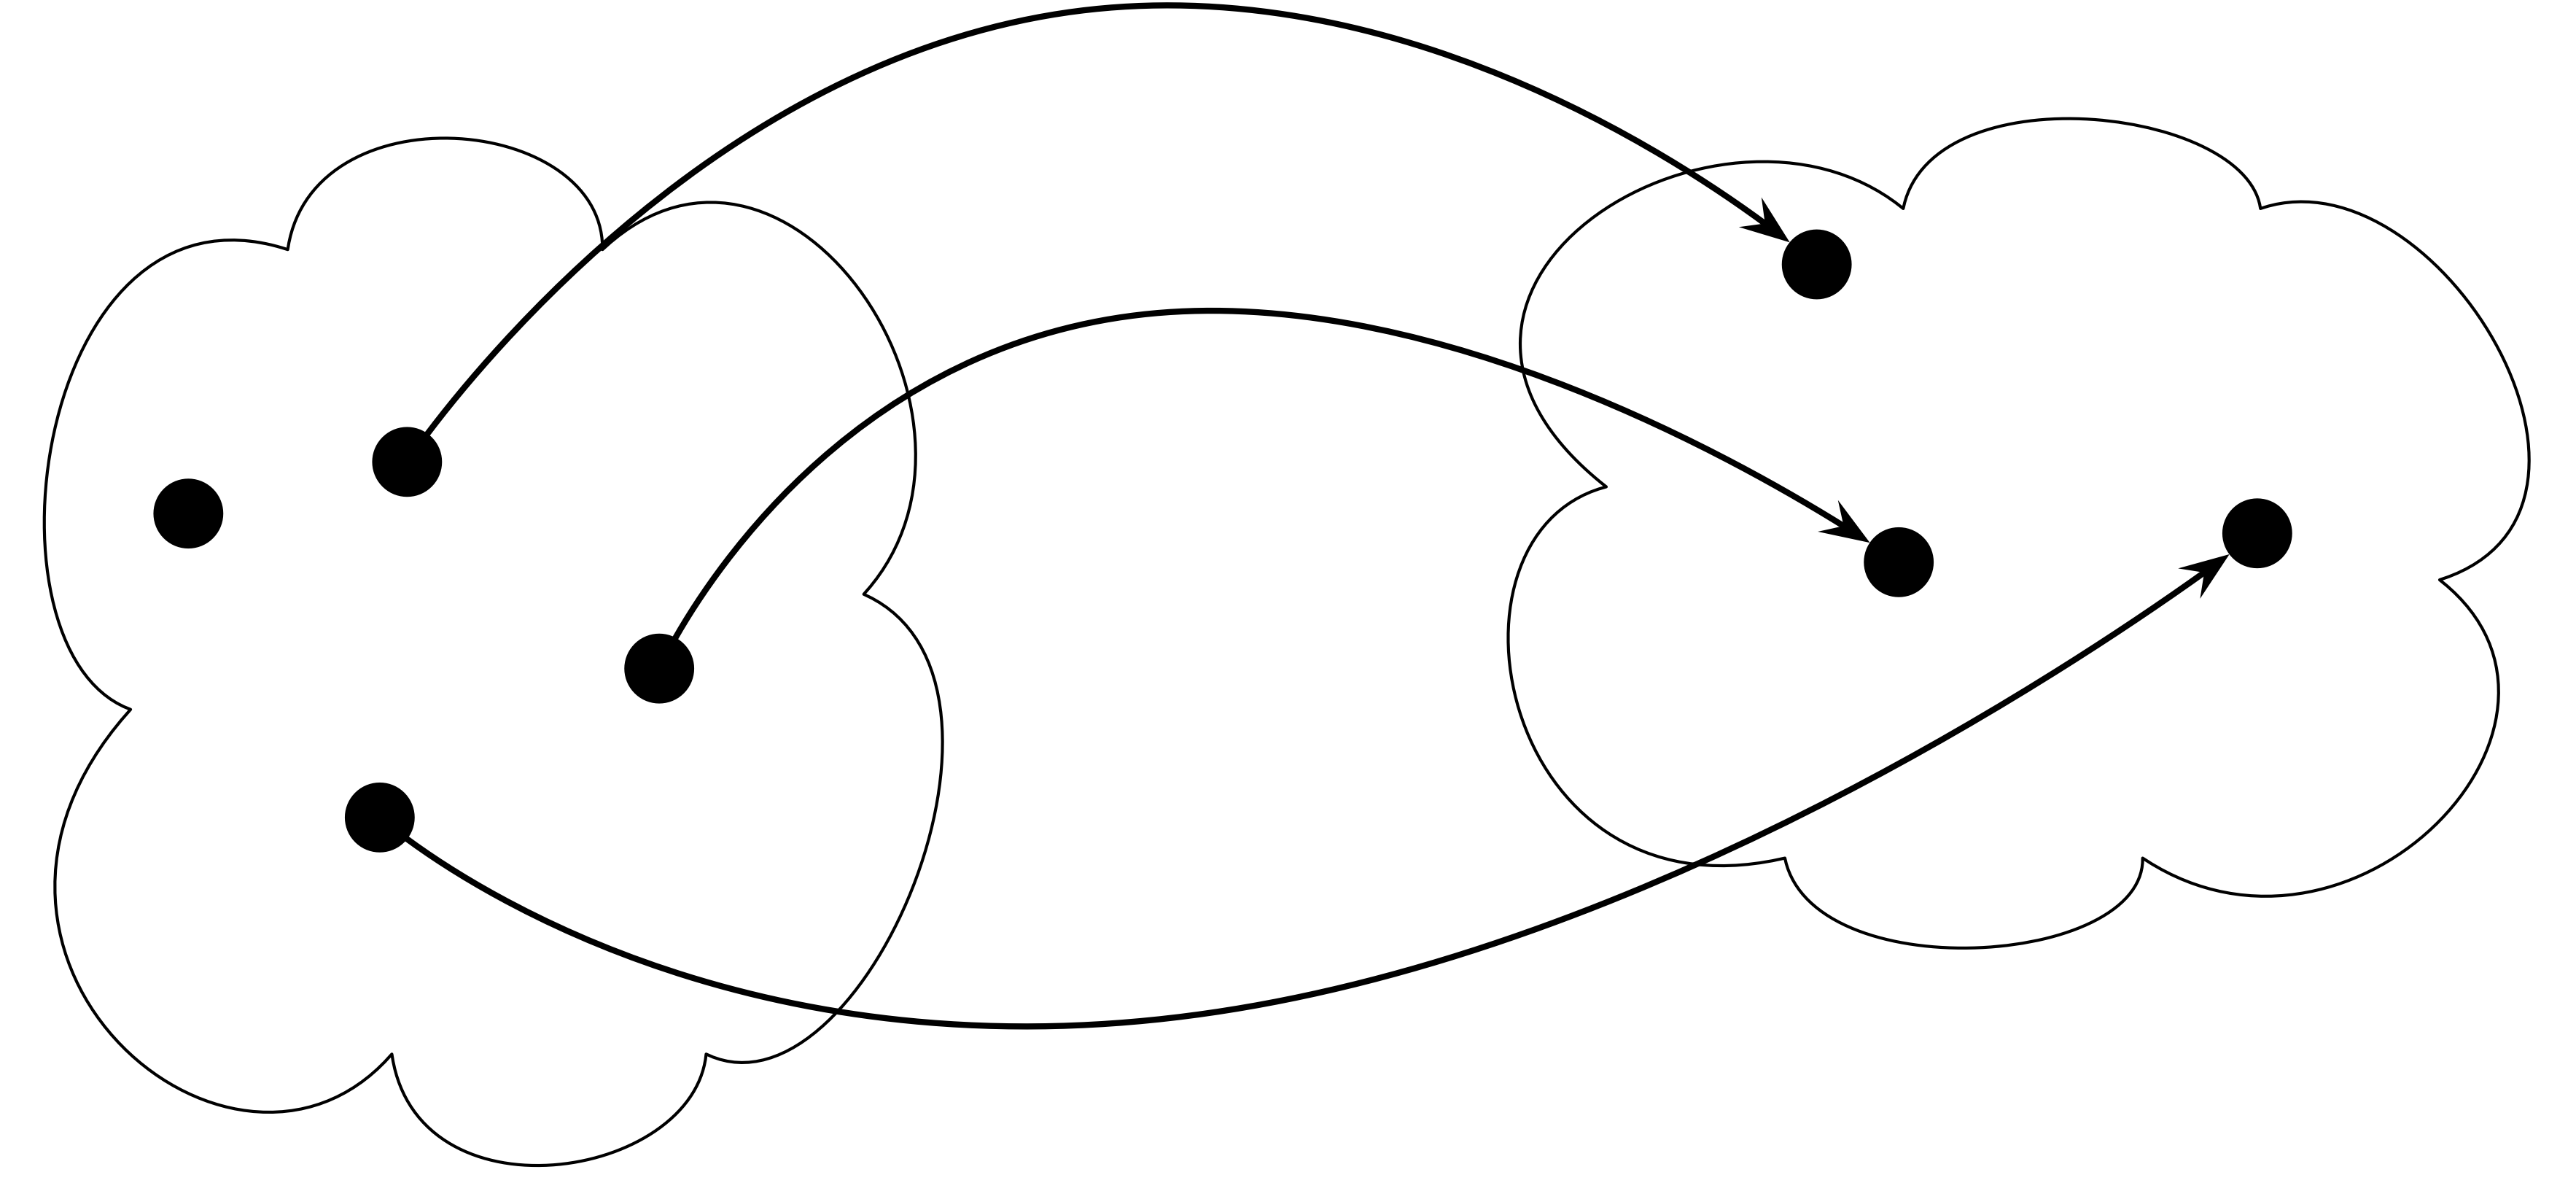
\includegraphics[width=.5\linewidth,right]{images/relations/surjection.png}
  \caption{Surjection.}
  \label{fig:surjection}
\end{figure}

\textbf{3.} The function \(f\) is a \textbf{bijection} if \(f\) is both injective and surjective. In other words, all elements of \(A\) are mapped uniquely to all elements of \(B\).

\begin{figure}
  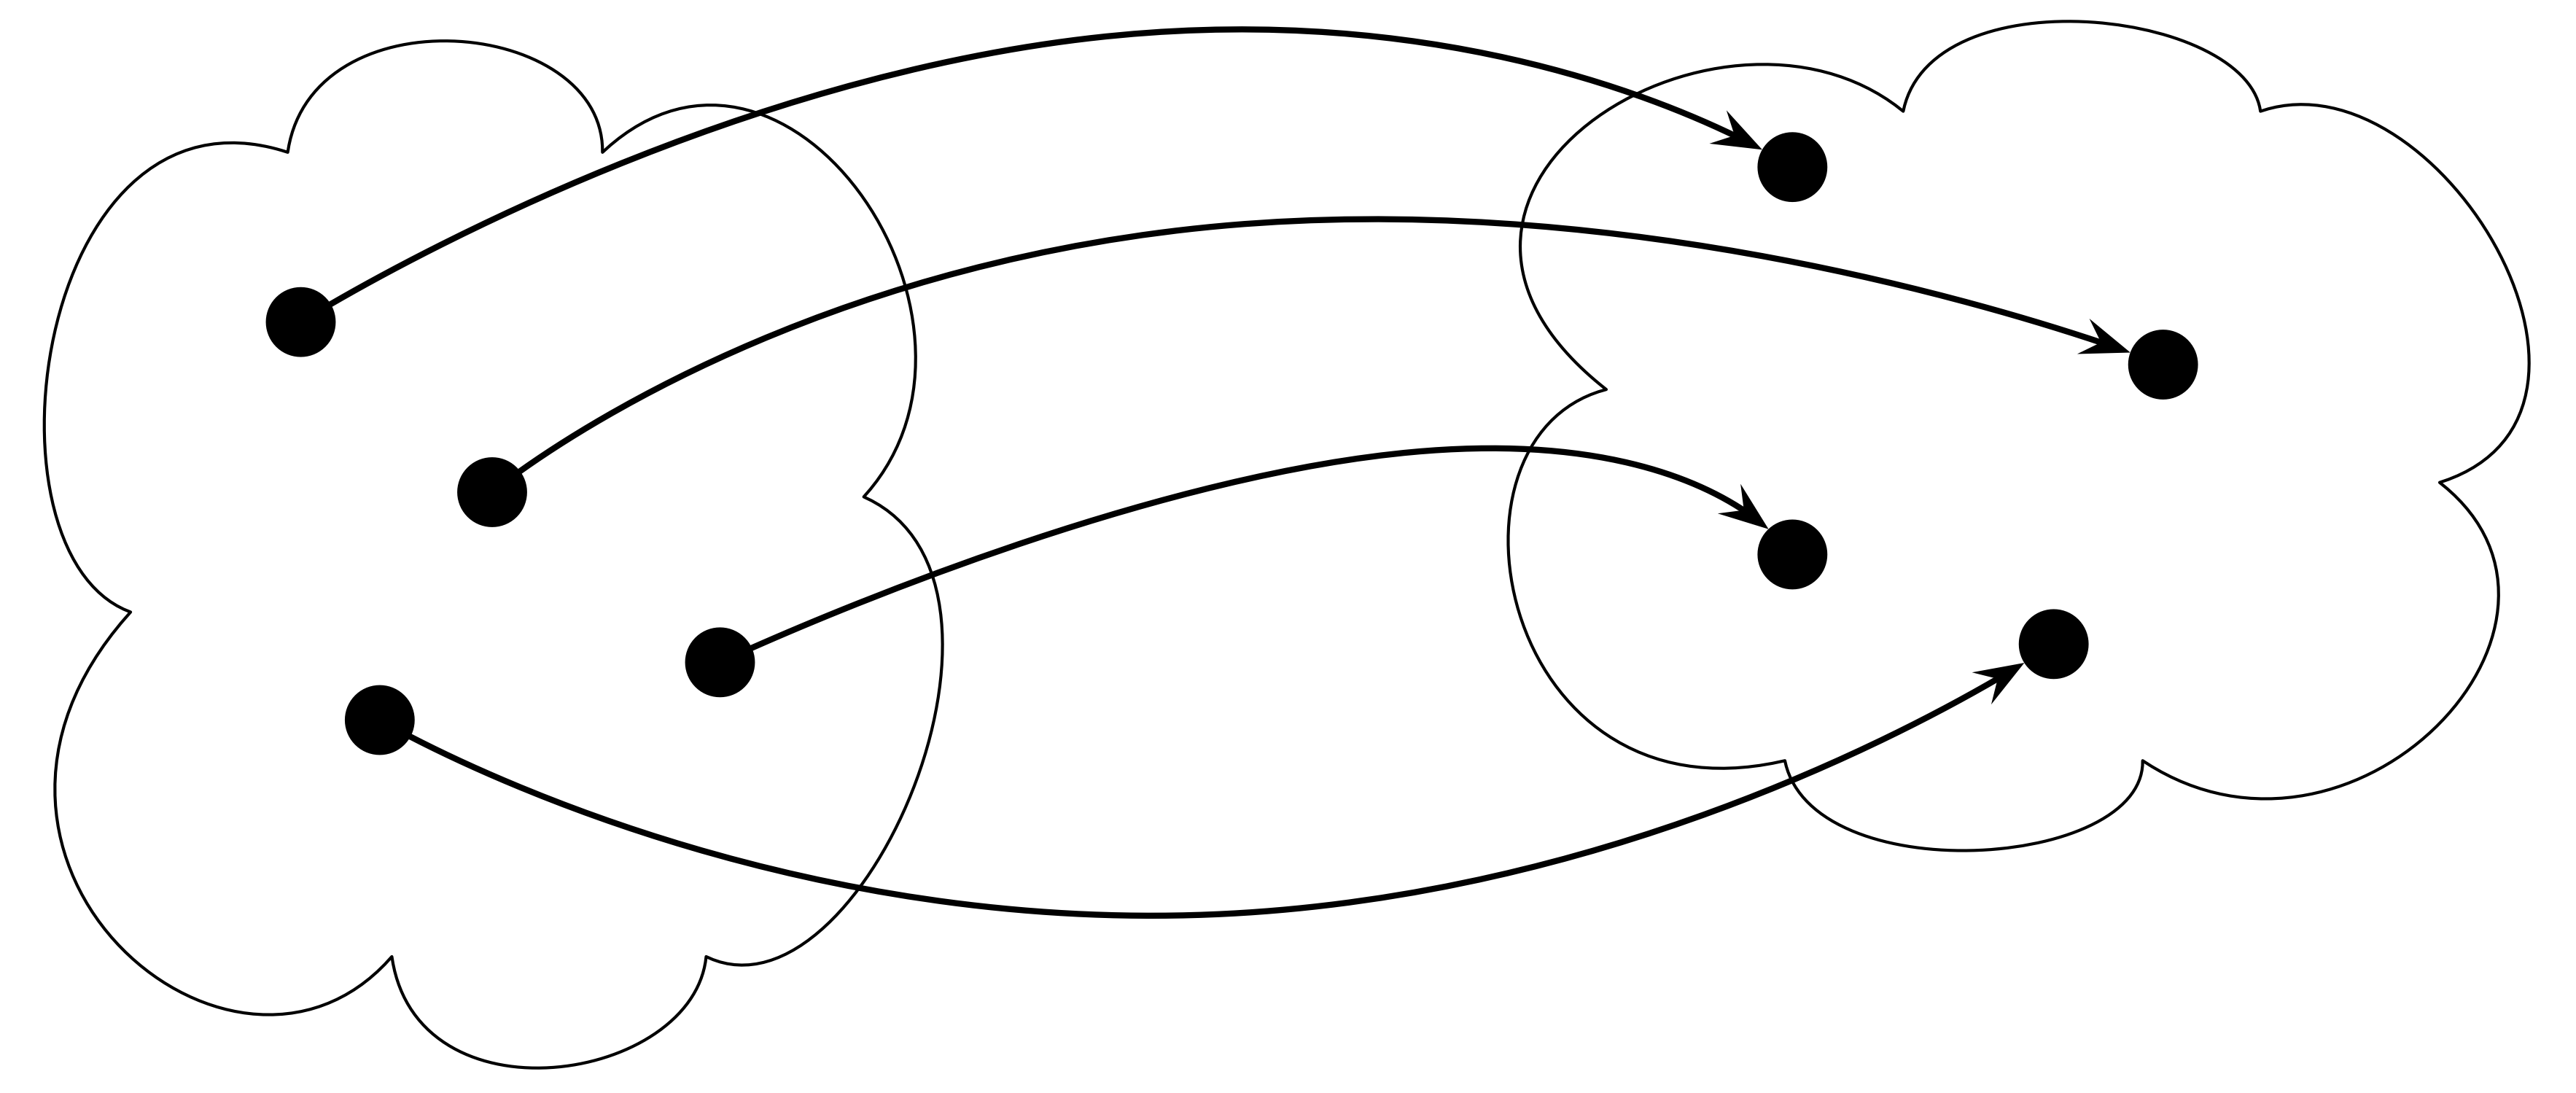
\includegraphics[width=.5\linewidth,right]{images/relations/bijection.png}
  \caption{Bijection.}
  \label{fig:bijection}
\end{figure}

We'll not focus on functions and relations anymore at the moment. Depending on how this course goes on, we'll either keep getting back to elements of this topic, or will extract it into a separate chapter.

\chapter{Proof techniques}
\label{sec:org5101666}

\section{Direct proof}
\label{sec:org39679d2}

Back when we were discussing set cardinality, we've successfully proved a statement: \emph{If \(A\) is a finite set of \(m\) elements, then there are \(2^{m}\) subsets of \(A\).} Let's talk about proofs in more detail, and discuss different proof techniques.

A proof is a sequence of mathematical statements, a path from some basic truth to the desired outcome. An impeccable argument, if you will. Possible the simplest form of proof is a direct proof. It's a direct attempt to see what the statement means if we dare to play with it. Consider a theorem:

\textbf{Theorem 1.} If \(n\) is an odd positive integer, then \(n^2\) is odd.

\textbf{Proof.} An odd positive integer can be written as \(n = 2k + 1\), since something like \(2k\) is even and adding 1 makes it definitely odd. We're interested in what odd squared looks like, so let's square this definition:

$$ n^2 = (2k + 1)^2 = $$
$$ 4k^2 + 4k + 1 = $$
$$ 2(2k^2 + 2k) + 1 $$

So, we have this final formula \(2(2k^2 + 2k) + 1\) and it follows the pattern of \(2k + 1\). This means it's odd! We have a proof.

This theorem is based on an idea that numbers described as \(2k + 1\) are definitely odd. This might be another theorem that requires another proof, and that proof might be based on some other theorems. The general idea of mathematics is that if you follow any theorem to the very beginning, you'll meet the fundamental axioms, the basis of everything.

\section{Constructive proof}
\label{sec:org71fb716}

The idea behind constructive proof is to prove the existence of a certain object by describing a method of creating it.

\textbf{Theorem 2.} There exists a rational number \(x\) such that \(\sqrt{10^{100}} < x < \sqrt{10^{100}+1}\).

\textbf{Proof.} \(\sqrt{10^{100}}\) is \(10^{50}\). Now, let's just try different clearly rational values for \(x\) that \emph{seem} to lie between the required boundaries. For example, let's try \(x = 10^{50} + 10^{51}\). It's obviously larger than \(10^{50}\), so we only need to show that it's smaller than \(\sqrt{10^{100}+1}\).

To do that, let's compute \(x^{2}\) so that we can compare it with \((\sqrt{10^{100}+1})^{2}\):

$$ x^{2} = ((10^{50} + 10^{-51})^{2} $$
$$ = 10^{100} + 2 \times (10^{50} \times 10^{-51}) + 10^{-102} $$
$$ = 10^{100} + 2 \times 10^{50-51} + 10^{-102} $$
$$ = 10^{100} + 2 \times 10^{-1} + 10^{-102} $$

Clearly, \(2 \times 10^{-1} + 10^{-102}\) is less than \(1\), so \(x^{2} < (\sqrt{10^{100}+1})^{2}\), and, by extension, \(x < \sqrt{10^{100}+1}\).

\section{Proof by Contradiction}
\label{sec:org3e7e6ab}

Another approach is proof by contradiction. Here is the idea:

\begin{enumerate}
\item Assume the statement is false or true.
\item Derive a contradiction, a paradox, something that doesn't make sense. This will mean that the statement cannot possibly be what we assumed it to be, therefore it's the opposite.
\end{enumerate}

When I first saw this formal technique, it puzzled me. It didn't seem to be valid: alright, assuming something is false leads to a paradox, so what? We haven't proven that assuming it's true doesn't lead to another paradox! Or even the same paradox, for that matter. What I failed to understand conceptually is that a statement is a binary thing: it's either true or untrue. Nothing in between. So, if one can definitely declare "X is not false", then no other options are left: "X must be true".

\textbf{Theorem 3.} \(n\) is a positive integer. If \(n^2\) is even, then \(n\) is even.

We may try to construct another direct proof, but creating paradoxes is much more fun!

\textbf{Proof.} Let's assume that \(n^2\) is even, \textbf{but \(n\) is odd}. This is the opposite of what we want, and we will show that this scenario is impossible.

\(n\) is odd, then, according to Theorem 3, \(n^2\) must be odd. This doesn't make sense! Our assumption and our conclusion are the opposite. This is a paradox, so the assumption was wrong. Meaning, the idea "\(n^2\) is even, but \(n\) is odd" is false. Therefore, the idea "\(n^2\) is even, \(n\) is even" is true.

\noindent\rule{\textwidth}{0.5pt}

\textbf{Theorem 4.} \(\sqrt{2}\) is irrational.

Woah, this is\ldots{} different. Prior theorems were formulas, something to play with, something physical. But here is just an idea, so how would we even start?

Let's start with a definition.

\begin{quote}
In mathematics, the irrational numbers are all real numbers which are not rational numbers.\footnote{\url{https://en.wikipedia.org/wiki/Irrational\_number}}
\end{quote}

Doesn't seem helpful, but let's continue. What are rational numbers then? Are they some reasonable beings who make optimal decisions all the time?

\begin{quote}
A rational number is any number that can be expressed as the fraction \(\frac{p}{q}\) of two integers.\footnote{\url{https://en.wikipedia.org/wiki/Rational\_number}}
\end{quote}

Oh! They are rational because they are \emph{ratios}! Just to make things super clear, let's dig one more step and make sure we understand integers.

\begin{quote}
An integer (from the Latin \emph{integer} meaning "whole") is a number that can be written without a fractional component. For example, \(21\), \(4\), \(0\), and \(−2048\) are integers, while \(9.75\), \(5\frac{1}{2}\) and \(\sqrt{2}\) are not.\footnote{\url{https://en.wikipedia.org/wiki/Integer}}
\end{quote}

Combining these things, we can construct a comprehensive definition of the irrational number: it's a number that cannot be expressed as the fraction of two whole numbers. Now, let's apply this to Theorem 3 so that it has some meat:

\textbf{Theorem 4, re-framed.} \(\sqrt{2}\) cannot be expressed as \(\frac{p}{q}\), where \(p\) and \(q\) are integers.

Alright, now there is something to play with!

\textbf{Proof.} Start by assuming the opposite -- \(\sqrt{2}\) is rational. This means it can be written as a fraction of two integers:

$$ \sqrt{2} = \frac{p}{q}\ $$

We can assume that \(p\) and \(q\) are not \textbf{both} even, because if they are, we can reduce them by dividing both by a common factor (like, for example, \(\frac{8}{10}\\) should be reduced to \(\frac{4}{5}\\)). In other words, if they are both even, reduce them until at least one is odd and no further reductions are possible.

Now, let's square the square root:

$$ (\sqrt{2})^2 = \frac{p^2}{q^2}\ $$

$$ 2 = \frac{p^2}{q^2}\ $$

$$ p^2 = 2q^2 $$

Remember, something like \(2k + 1\) is odd, and \(2k\) is even. Here we see this pattern: \(p^2 = 2q^2\), which means that \(p^2\) is even (it consists of \emph{two} things).

Then, using Theorem 3, we can say that \(p\) is even as well, which means we can write \(p\) as \(p = 2k\). So:

$$ 2q^2 = p^2 = (2k)^2 $$

$$ 2q^2 = 4k^2 $$

Divide both by two:

$$ q^2 = 2k^2 $$

So, \(q^2\) is even. By the same Theorem 2 it follows that \(q\) is even.

Let's summarize the two conclusions:

\begin{enumerate}
\item \(p\) is even.
\item \(q\) is even.
\end{enumerate}

Wait\ldots{} We made sure that not both \(p\) and \(q\) are even before starting this whole thing! We made sure to reduce them until at least one is odd, but then, by applying Theorem 2, we ended up with two even numbers. This is impossible, so the idea that "\(\sqrt{2}\) is rational" is not true.

Therefore, \(\sqrt{2}\) is irrational.

\section{Proof by Induction}
\label{sec:orgfa77e48}

One of the most powerful techniques is proof by induction.

\marginnote{Do not confuse mathematical induction with inductive or deductive reasoning. Despite the name, mathematical induction is actually a form of deductive reasoning.}

Let's say, we want to prove that some statement \(P\) is true for all positive integers. In other words:

\(P(1)\) is true, \(P(2)\) is true, \(P(3)\) is true\ldots{} etc.

We could try and prove each one directly or by contradiction, but the infinite number of positive integers makes this task rather grueling. Proof by induction is a sort of generalization that starts with the basis:

\textbf{Basis:} Prove that \(P(1)\) is true.

Then makes one generic step that can be applied indefinitely:

\textbf{Induction step:} Prove that for all \(n\geq1\), the following statement holds: If \(P(n)\) is true, then \(P(n+1)\) is also true.

We've devised another problem to solve, and it's seemingly the same. But if the basis is true, then proving this \emph{inductive step} will prove the theorem. To do this, we chose an arbitrary \(n\geq1\) and assumed that \(P(n)\) is true. This assumption is called the \emph{inductive hypothesis}. The tricky part is this: we don't prove the hypothesis directly, but prove the \(n+1\) version of it.

This is all rather amorphous, so let's prove a real theorem.

\textbf{Theorem 5.} For all positive integers \(n\), the following is true:

\begin{equation}
\label{eq:1}
1 + 2 + 3 + ... + n = \frac{n(n+1)}{2}
\end{equation}

\textbf{Proof}. Start with the basis when \(n\) is \(1\). Just calculate it:

$$ 1 = \frac{1(1+1)}{2}. $$

This is correct, so, the basis is proven. Now, assume that the theorem is true for any \(n\geq1\):

\begin{equation}
\label{eq:2}
1 + 2 + 3 + ... + n = \frac{n(n+1)}{2}
\end{equation}

In the induction step we have to prove that it's true for \(n+1\):

\begin{equation}
\label{eq:3}
1 + 2 + 3 + ... + (n+1) = \frac{(n+1)(n+2)}{2}
\end{equation}


Having this equation, we should just try to expand it and prove directly. Since the last member on the left side is \(n+1\), the second last must be \(n\), so:

$$ 1 + 2 + 3 + ... + (n + 1) = 1 + 2 + 3 + ... + n + (n+1) $$

From our assumption, we know, that

$$ 1 + 2 + 3 + ... + n = \frac{n(n+1)}{2}. $$

So, let's replace it on the right hand side:

$$ 1 + 2 + 3 + ... + (n + 1) = \frac{n(n+1)}{2} + (n+1) $$

And then make that addition so that the right hand side is a single fraction:

$$ 1 + 2 + 3 + ... + (n + 1) = \frac{n(n+1)}{2} + \frac{2(n+1)}{2} $$

$$ = \frac{n(n+1) + 2(n+1)}{2} $$

$$ = \frac{(n+1)(n+2)}{2}. $$

Done, we have proven that the inductive step (\ref{eq:3}) is true.

There are two results:

\begin{enumerate}
\item The theorem is true for \(n=1\).
\item If the theorem is true for any \(n\), then it's also true for \(n+1\).
\end{enumerate}

Combining these two results we can conclude that the theorem is true for all positive integers \(n\).

\noindent\rule{\textwidth}{0.5pt}

I had troubles with this technique because for a long time I couldn't for the life of me understand why is this \emph{enough} and how is the basis \emph{helping}?! The basis seemed redundant. We assume \(P(n)\) is true, then prove that \(P(n+1)\) is true given that \(P(n)\) is true, but so what? We didn't prove the thing we assumed!

It clicked after I understood that we don't have to prove \(P(n)\), we just take the concrete value from the basis and use it as \(n\). Since we have a proof of \(P(n+1)\) being true \textbf{if} \(P(n)\) is true, we conclude that if \(P(1)\) is true, then \(P(1+1)\) is true.

Well, if \(P(1+1)\) is true, then, using the same idea, \(P(1+1+1)\) is true, and so forth.

The basis was the cheat-code to kick-start the process by avoiding the need to prove the assumption \ref{eq:2}.

\section{The pigeon hole principle}
\label{sec:org2d96568}
\end{document}
